% ------------------------------------------------------------------------------
% TYPO3 CMS 6.2 LTS - What's New (Spanish Version)
%
% @author	Sergio Catalá <sergio.catala@e-net.info>
% @author	Michel Mix <mmix@autistici.org>
% @license	Creative Commons BY-NC-SA 3.0
% @link		http://typo3.org/download/release-notes/whats-new/
% @language	Spanish
% ------------------------------------------------------------------------------

% change the default aspect ratio and frame size
% \documentclass[aspectratio=43]{beamer}
%
% specify vertical top alignment globally by the [t] class option:
% \documentclass[t]{beamer}
%
% for single frames, use the same option locally:
% \begin{frame}[t] ... \end{frame}

\documentclass[t]{beamer}

% suppress navigation bar
\beamertemplatenavigationsymbolsempty

\mode<presentation>
{
	\usetheme{typo3slides}
}

% global variables
\title{TYPO3 CMS 6.2 LTS - Qué hay Nuevo}
\subtitle{Resumen de las nuevas características, cambios y mejoras}
\author{
	\centerline{Creado por:}
	\centerline{Patrick Lobacher y Michael Schams}
	\vspace{0.4cm}
	\centerline{Traducción en Español por:}
	\centerline{Sergio Catalá y Michel Mix}
}
\date{\today}

\begin{document}

% select TYPO3 Share font
\sharefont

% ------------------------------------------------------------------------------
% Title Page
% ------------------------------------------------------------------------------

\begingroup
	\setbeamercolor{normal text}{fg=white,bg=typo3orange}
	\setbeamercolor{title}{fg=white}
	\setbeamercolor{author}{fg=white}
	\setbeamertemplate{footline}[default]
	\begin{frame}
		\titlepage
	\end{frame}
\endgroup

% ------------------------------------------------------------------------------
% Table of Contents
% ------------------------------------------------------------------------------

% between two frames: use \newpage (not \clearpage!) to force a column break:
% \addtocontents{toc}{\newpage}

\section*{TYPO3 CMS 6.2 LTS - Qué hay Nuevo}
\begin{frame}[fragile]
	\frametitle{Resumen de Capítulos}
	\framesubtitle{Resumen de Capítulos}

	\begin{multicols}{2}
		\tableofcontents
	\end{multicols}

\end{frame}

% ------------------------------------------------------------------------------
% Chapter: Introduction
% ------------------------------------------------------------------------------

% ------------------------------------------------------------------------------
% TYPO3 CMS 8.4 - What's New - Chapter "Introduction" (Italian Version)
%
% @author	Michael Schams <schams.net>
% @license	Creative Commons BY-NC-SA 3.0
% @link		http://typo3.org/download/release-notes/whats-new/
% @language	English
% ------------------------------------------------------------------------------
% LTXE-CHAPTER-UID:		7fdf26cc-362160ab-d6c8b905-19722b20
% LTXE-CHAPTER-NAME:	Introduction
% ------------------------------------------------------------------------------

\section{Introduzione}
\begin{frame}[fragile]
	\frametitle{Introduzione}

	\begin{center}\huge{Introduzione}\end{center}
	\begin{center}\huge{\color{typo3darkgrey}\textbf{I fatti in breve}}\end{center}

\end{frame}

% ------------------------------------------------------------------------------
% LTXE-SLIDE-START
% LTXE-SLIDE-UID:		36bbd1e7-b70470c2-e4557331-e851ab9a
% LTXE-SLIDE-ORIGIN:	344cc625-72176049-0721f1aa-0580f11a English
% LTXE-SLIDE-TITLE:		TYPO3 CMS 8.4 - The Facts
% ------------------------------------------------------------------------------
\begin{frame}[fragile]
	\frametitle{Introduzione}
	\framesubtitle{TYPO3 CMS 8.4 - I fatti in breve}

	\begin{itemize}
		\item Data di rilascio: 18 Ottobre 2016
		\item Tipo di rilascio: Sprint Release
		\item Slogan: Fueling
	\end{itemize}

	\begin{figure}
		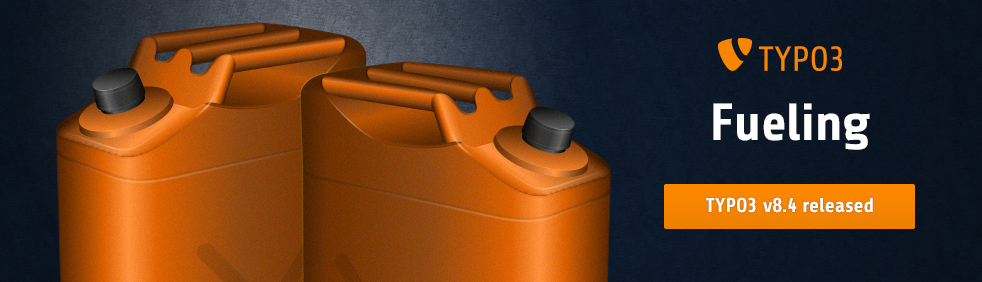
\includegraphics[width=0.95\linewidth]{Introduction/typo3cms84-banner.jpg}
	\end{figure}

\end{frame}

% ------------------------------------------------------------------------------
% LTXE-SLIDE-START
% LTXE-SLIDE-UID:		c34db54f-5ce84e64-993b5283-bd1414c5
% LTXE-SLIDE-ORIGIN:	59b04868-09a761b3-0c7ca4c3-ce6e31bb English
% LTXE-SLIDE-TITLE:		System Requirements
% ------------------------------------------------------------------------------
\begin{frame}[fragile]
	\frametitle{Introduzione}
	\framesubtitle{Requisiti di sistema}

	\begin{itemize}
		\item PHP:\tabto{2.2cm}versione 7
		\item MySQL:\tabto{2.2cm}versione da 5.5 a 5.7
		\item Spazio disco:\tabto{2.2cm}min 200 MB
		\item Impostazioni PHP:

			\begin{itemize}
				\item \texttt{memory\_limit} >= 128M
				\item \texttt{max\_execution\_time} >= 240s
				\item \texttt{max\_input\_vars} >= 1500
				\item l'opzione di compilazione \texttt{-}\texttt{-disable-ipv6} \underline{non} deve essere usata
			\end{itemize}

		\item Il Backend richiede Microsoft Internet Explorer 11 o superiore,
			Microsoft Edge, Google Chrome, Firefox, Safari o altro browser recente
			e compatibile

	\end{itemize}

\end{frame}

% ------------------------------------------------------------------------------
% LTXE-SLIDE-START
% LTXE-SLIDE-UID:		6d7a088e-555bc078-1d2027f1-5046d232
% LTXE-SLIDE-ORIGIN:	41f1b51a-6b837f9d-c4aa9584-66f8e47f English
% LTXE-SLIDE-TITLE:		Development And Release Timeline
% ------------------------------------------------------------------------------
\begin{frame}[fragile]
	\frametitle{Introduzione}
	\framesubtitle{Sviluppo e tempi di rilascio}

	\begin{figure}
		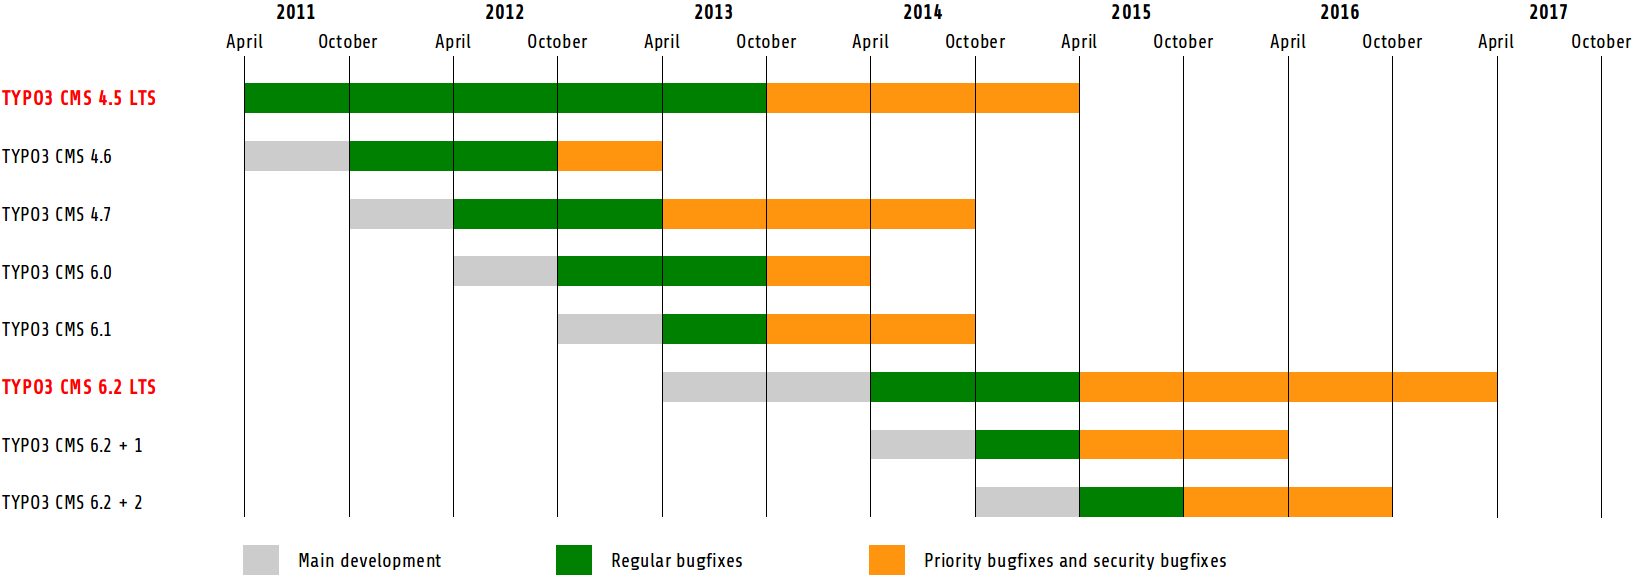
\includegraphics[width=1\linewidth]{Introduction/ReleaseAgenda.png}
	\end{figure}

\end{frame}

% ------------------------------------------------------------------------------
% LTXE-SLIDE-START
% LTXE-SLIDE-UID:		ef57635b-0d6818d0-bc469ed4-3c810ae4
% LTXE-SLIDE-ORIGIN:	f7c981ac-f359aac8-f8799a73-2adc6532 English
% LTXE-SLIDE-TITLE:		TYPO3 CMS Roadmap
% ------------------------------------------------------------------------------
\begin{frame}[fragile]
	\frametitle{Introduzione}
	\framesubtitle{TYPO3 CMS Roadmap}

	Date di rilascio stimate e loro obiettivo principale:

	\begin{itemize}

		\item v8.0 \tabto{1.1cm}22/Mar/2016\tabto{3.4cm}Aggiunta di parti dell'ultimo momento
		\item v8.1 \tabto{1.1cm}03/Mag/2016\tabto{3.4cm}Integrazione cloud
		\item v8.2 \tabto{1.1cm}05/Lug/2016\tabto{3.4cm}Prerequisiti Doctrine
		\item v8.3 \tabto{1.1cm}30/Ago/2016\tabto{3.4cm}Rich Text Editor
		\item
			\begingroup
				\color{typo3orange}
					v8.4 \tabto{1.1cm}18/Ott/2016\tabto{3.4cm}Migrazione Doctrine + Aggiornamenti
			\endgroup
		\item v8.5 \tabto{1.1cm}20/Dic/2016\tabto{3.4cm}Nuovo RTE + Supporto Integrazione
		\item v8.6 \tabto{1.1cm}14/Feb/2017\tabto{3.4cm}\textit{da determinare}
		\item v8.7 \tabto{1.1cm}04/Apr/2017\tabto{3.4cm}Preparazione LTS

	\end{itemize}

	\smaller
		\url{https://typo3.org/typo3-cms/roadmap/}\newline
		\url{https://typo3.org/news/article/kicking-off-typo3-v8-development/}
	\normalsize

\end{frame}

% ------------------------------------------------------------------------------
% LTXE-SLIDE-START
% LTXE-SLIDE-UID:		df4f964f-fa8cb997-19c5170a-4dc9c6b2
% LTXE-SLIDE-ORIGIN:	425f3f15-1178ed7e-f26438f9-a79ad9e9 English
% LTXE-SLIDE-TITLE:		Installation
% ------------------------------------------------------------------------------
\begin{frame}[fragile]
	\frametitle{Introduzione}
	\framesubtitle{Installazione}

	\begin{itemize}
		\item Procedura ufficiale di installazione su Linux/Mac OS X\newline
			(Directory Root ad esempio \texttt{/var/www/site/htdocs}):
		\begin{lstlisting}
			$ cd /var/www/site
			$ wget --content-disposition get.typo3.org/8.4
			$ tar xzf typo3_src-8.4.1.tar.gz
			$ cd htdocs
			$ ln -s ../typo3_src-8.4.1 typo3_src
			$ ln -s typo3_src/index.php
			$ ln -s typo3_src/typo3
			$ touch FIRST_INSTALL
		\end{lstlisting}

		\item Link simbolici in Microsoft Windows:

			\begin{itemize}
				\item Usa \texttt{junction} in Windows XP/2000
				\item Usa \texttt{mklink} in Windows Vista e Windows 7
			\end{itemize}

	\end{itemize}
\end{frame}

% ------------------------------------------------------------------------------
% LTXE-SLIDE-START
% LTXE-SLIDE-UID:		e38ae238-c1d61e71-6406f3e1-8f93121d
% LTXE-SLIDE-ORIGIN:	061ecffe-6aadad2d-6e64a67a-3c50a5cf English
% LTXE-SLIDE-TITLE:		Upgrade to TYPO3 CMS 7
% ------------------------------------------------------------------------------
\begin{frame}[fragile]
	\frametitle{Introduzione}
	\framesubtitle{Aggiornamento a TYPO3 CMS 8.x}

	\begin{itemize}
		\item Aggiornamenti possibili solo da TYPO3 CMS 7.6 LTS
		\item TYPO3 CMS < 7.6 LTS deve essere prima aggiornato a TYPO3 CMS 7.6 LTS
	\end{itemize}

	\begin{itemize}

		\item Istruzioni per l'aggiornamento:\newline
			\smaller\url{http://wiki.typo3.org/Upgrade#Upgrading_to_8.3}\normalsize
		\item Guida ufficiale TYPO3 "TYPO3 Installation and Upgrading":
			\smaller\url{http://docs.typo3.org/typo3cms/InstallationGuide}\normalsize
		\item Approcio generale:
			\begin{itemize}
				\item Verifica i requisiti minimi di sistema \small(PHP, MySQL, etc.)
				\item Verifica \textbf{deprecation\_*.log} nella vecchia istanza TYPO3
				\item Aggiorna tutte le estensioni all'ultima versione
				\item Imposta il nuovo sorgente ed esegui Install Tool -> Upgrade Wizard
				\item Verifica il modulo di startup per gli utenti di backend (opzionale)
			\end{itemize}
	\end{itemize}

\end{frame}

% ------------------------------------------------------------------------------

% ------------------------------------------------------------------------------
% LTXE-SLIDE-START
% LTXE-SLIDE-UID:		5449eaf9-054a9da9-8cccada5-eb6655ca
% LTXE-SLIDE-ORIGIN:	560abc87-898d82d3-b9e35f84-e348c121 English
% LTXE-SLIDE-TITLE:		PHP Version 7
% ------------------------------------------------------------------------------
\begin{frame}[fragile]
	\frametitle{Introduzione}
	\framesubtitle{PHP Version 7}

	\begin{itemize}

		\item PHP 7.0 è un requisito minimo per TYPO3 CMS 8.x
		\item TYPO3 supporterà i successivi rilasci di PHP 7 mano a mano che saranno pubblicati
		\item Questa versione fornisce un significativo incremento delle prestazioni del sistema

		\item Non solo gli editori di backend noteranno un interfaccia più veloce, ma il tempo
			di caricamento di un intera pagina di frontend in cache è inferiore a
			7 millisecondi, che è circa il 40\% più veloce paragonandolo
			allo stesso sito web con PHP versione 5.5

		\item Si sono iniziate ad utilizzare anche le nuove funzioni di questa versione di PHP,
			per esempio i generatori crittografici pseudo-casuali sono già in uso.

	\end{itemize}

\end{frame}

% ------------------------------------------------------------------------------


% ------------------------------------------------------------------------------
% Chapter 1: Install Tool
% ------------------------------------------------------------------------------

% ------------------------------------------------------------------------------
% TYPO3 CMS 6.2 LTS - What's New - Chapter "Install Tool" (English Version)
%
% @author	Michael Schams <schams.net>
% @license	Creative Commons BY-NC-SA 3.0
% @link		http://typo3.org/download/release-notes/whats-new/
% @language	English
% ------------------------------------------------------------------------------
% Chapter: Install Tool
% ------------------------------------------------------------------------------

\section{Install Tool}
\begin{frame}[fragile]
	\frametitle{Install Tool}

	\begin{center}\huge{Chapter 1:}\end{center}
	\begin{center}\huge{\color{typo3darkgrey}\textbf{The Install Tool}}\end{center}

\end{frame}

% ------------------------------------------------------------------------------
% Installation
% ------------------------------------------------------------------------------

\begin{frame}[fragile]
	\frametitle{Install Tool}
	\framesubtitle{Installation}

	\begin{itemize}
		\item Only \underline{one} package is required for an installation:\newline
				\texttt{typo3\_src-6.2.x.tar.gz} (file size: approx. 20MB)
		\item "Dummy" and "Blank" packages became obsolete
		\item Installation:
			\begin{itemize}
				\item Extract source package into web root directory
				\item Create symbolic links as required
				\item Point web browser to your web root
				\item TYPO3 Installer starts 1-2-3-4-5-steps wizard
			\end{itemize}

	\end{itemize}

\end{frame}

% ------------------------------------------------------------------------------
% Installation
% ------------------------------------------------------------------------------

\begin{frame}[fragile]

	\frametitle{Install Tool}
	\framesubtitle{Installation}

	\begin{itemize}
		\item Installer ensures that all required files and directories are in place
		\item Files required for a custom setup will be created automatically
		\item The following symbolic links \underline{must} exist:

		\begin{itemize}
			\item \texttt{typo3\_src}	\tabto{2cm} (points to TYPO3 source directory)
			\item \texttt{typo3}		\tabto{2cm} (points to directory: \texttt{typo3\_src/typo3})
			\item \texttt{index.php}	\tabto{2cm} (points to file: \texttt{typo3\_src/index.php})
		\end{itemize}

		\item No further files/directories are required to install TYPO3!
		\item Directory \texttt{t3lib} removed
		\item Further details: TYPO3 Installation and Upgrade Guide\newline
			\url{http://docs.typo3.org/typo3cms/InstallationGuide}

	\end{itemize}

\end{frame}

% ------------------------------------------------------------------------------
% Re-Development
% ------------------------------------------------------------------------------

\begin{frame}[fragile]
	\frametitle{Install Tool}
	\framesubtitle{Re-Development}

	\begin{columns}[T]

		\begin{column}{.5\textwidth}
			\begin{itemize}
				\item Re-developed from scratch\newline using Fluid
				\item \underline{First} step tests system environment and reports issues
				\item Reported issues can be fixed\newline (and re-tested) or ignored
				\item Invalid core setup (e.g. no symbolic links as recommended) is reported as an issue, too
			\end{itemize}
		\end{column}

		\begin{column}{.5\textwidth}
			\begin{figure}\vspace*{-0.4cm}
				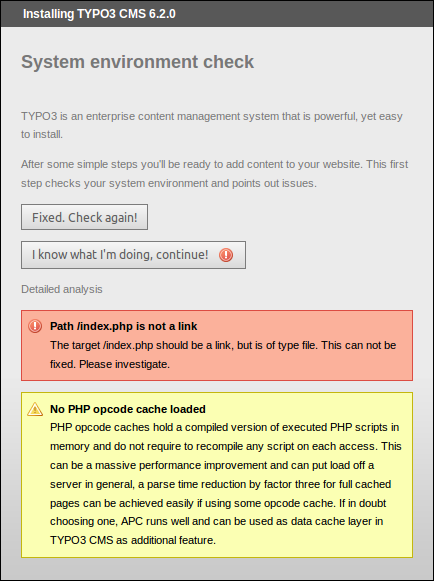
\includegraphics[width=0.8\linewidth]{Images/InstallTool/SystemEnvironmentCheck.png}
			\end{figure}
		\end{column}

	\end{columns}

\end{frame}

% ------------------------------------------------------------------------------
% Re-Development
% ------------------------------------------------------------------------------

\begin{frame}[fragile]
	\frametitle{Install Tool}
	\framesubtitle{Re-Development}

	\begin{columns}[T]

		\begin{column}{.5\textwidth}
			\begin{itemize}
				\item \underline{Second} step allows users to enter database access details
				\item Connection types are selectable
					\begin{itemize}
						\item TCP/IP based connection
						\item Socket based connection
					\end{itemize}
				\item MySQL alternatives are also possible
			\end{itemize}
		\end{column}

		\begin{column}{.5\textwidth}
			\begin{figure}\vspace*{-0.4cm}
				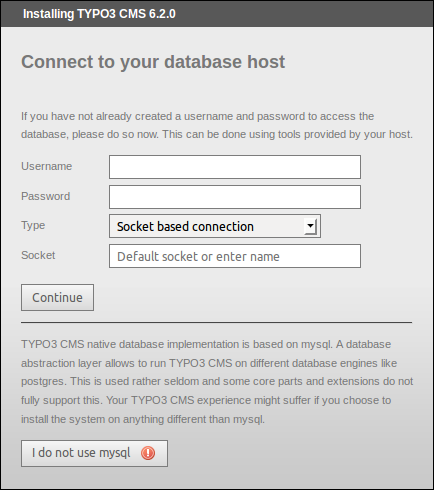
\includegraphics[width=0.8\linewidth]{Images/InstallTool/DatabaseConnectionDetails.png}
			\end{figure}
		\end{column}

	\end{columns}

\end{frame}

% ------------------------------------------------------------------------------
% Re-Development
% ------------------------------------------------------------------------------

\begin{frame}[fragile]
	\frametitle{Install Tool}
	\framesubtitle{Re-Development}

	\begin{columns}[T]

		\begin{column}{.5\textwidth}
			\begin{itemize}
				\item \underline{Third} step allows users to select/create the database\newline
					(as in TYPO3 < 6.2)
				\item \underline{Fourth} step allows users to set a password for the "admin" user\newline (which is also the initial Install Tool password) and a site name
			\end{itemize}
		\end{column}

		\begin{column}{.5\textwidth}
			\begin{figure}\vspace*{-0.4cm}
				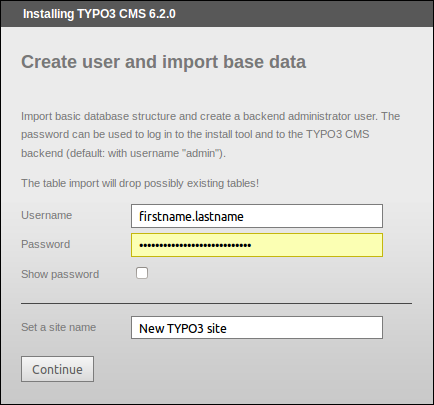
\includegraphics[width=0.8\linewidth]{Images/InstallTool/AdminPasswordAndSiteName.png}
			\end{figure}
		\end{column}

	\end{columns}

\end{frame}

% ------------------------------------------------------------------------------
% Clear All Cache
% ------------------------------------------------------------------------------

\begin{frame}[fragile]
	\frametitle{Install Tool}
	\framesubtitle{Clear All Cache}

	\begin{itemize}
		\item New function under "Important actions" lets users clear all cache
		\item This also works, if cache contains invalid PHP code\newline
			(which possibly locks TYPO3 CMS)
		\item Bypass a not-working TYPO3 instance by accessing the Install Tool directly: \texttt{http://example.com/typo3/install}
	\end{itemize}

	\begin{columns}[T]
		\begin{column}{.3\textwidth}
			\begin{figure}\vspace*{-0.4cm}
				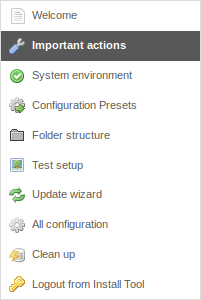
\includegraphics[width=0.7\linewidth]{Images/InstallTool/ImportantActions.png}
			\end{figure}
		\end{column}
		\begin{column}{.7\textwidth}
			\begin{figure}\vspace*{-0.4cm}
				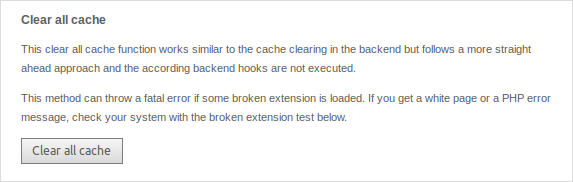
\includegraphics[width=0.9\linewidth]{Images/InstallTool/ClearAllCache.png}
			\end{figure}
		\end{column}
	\end{columns}

\end{frame}

% ------------------------------------------------------------------------------
% Clear All Cache
% ------------------------------------------------------------------------------

\begin{frame}[fragile]
	\frametitle{Install Tool}
	\framesubtitle{Clear All Cache}

	Sequence of actions when executing "Clear all cache":

	\begin{enumerate}
		\item Content of directory \texttt{typo3temp/Cache} is deleted
		\item Database tables \texttt{cf\_*} are emptied
		\item Files \texttt{ext\_localconf.php} and \texttt{ext\_tables.php}\newline
			are loaded from extensions
		\item \texttt{flushCaches()} are executed
	\end{enumerate}

\end{frame}

% ------------------------------------------------------------------------------
% Check For Broken Extensions
% ------------------------------------------------------------------------------

\begin{frame}[fragile]
	\frametitle{Install Tool}
	\framesubtitle{Check For Broken Extensions}

	\begin{itemize}
		\item New function under "Important actions" lets users check,\newline
			if extensions can be loaded without breaking the system
		\item Very useful for an update from TYPO3 4.5 to 6.2
	\end{itemize}

	\begin{columns}[T]
		\begin{column}{.3\textwidth}
			\begin{figure}\vspace*{-0.4cm}
				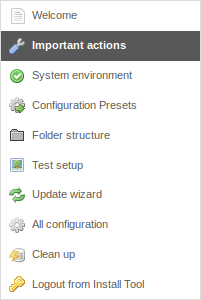
\includegraphics[width=0.7\linewidth]{Images/InstallTool/ImportantActions.png}
			\end{figure}
		\end{column}
		\begin{column}{.7\textwidth}
			\begin{figure}\vspace*{-0.4cm}
				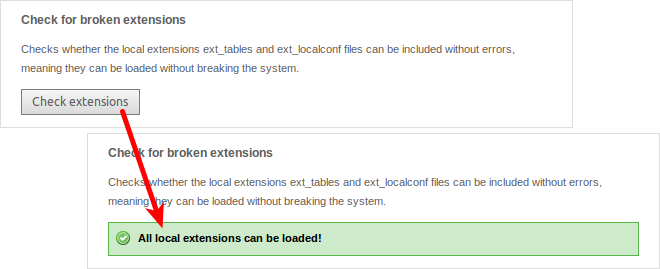
\includegraphics[width=1\linewidth]{Images/InstallTool/CheckForBrokenExtensions.png}
			\end{figure}
		\end{column}
	\end{columns}

\end{frame}

% ------------------------------------------------------------------------------
% Increased Security: Salted Passwords
% ------------------------------------------------------------------------------

\begin{frame}[fragile]
	\frametitle{Install Tool}
	\framesubtitle{Salted Passwords}

	\begin{itemize}
		\item When creating new backend administrator user via Install Tool,\newline
			a \textbf{salted} password is used\newline
			\smaller(requires installed, loaded and configured EXT:saltedpasswords)\normalsize
		\item Install Tool password is a \textbf{salted} password as well\newline
			\smaller(existing MD5 hashes are converted automatically at first login)\normalsize
	\end{itemize}

	\begin{columns}[T]
		\begin{column}{.3\textwidth}
			\begin{figure}\vspace*{-0.4cm}
				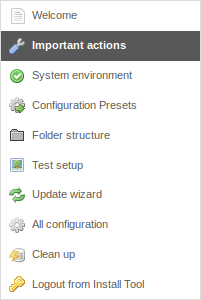
\includegraphics[width=0.7\linewidth]{Images/InstallTool/ImportantActions.png}
			\end{figure}
		\end{column}
		\begin{column}{.7\textwidth}
			\begin{figure}\vspace*{-0.4cm}
				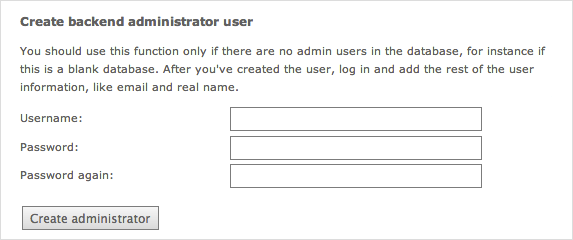
\includegraphics[width=0.9\linewidth]{Images/InstallTool/SaltedPasswords.png}
			\end{figure}
		\end{column}
	\end{columns}

\end{frame}

% ------------------------------------------------------------------------------
% Application Context
% ------------------------------------------------------------------------------

\begin{frame}[fragile]
	\frametitle{Install Tool}
	\framesubtitle{Application Context (1)}

	\begin{itemize}
		\item TYPO3 >= 6.2 takes \textbf{Application Context} into account\newline
			\smaller(known from TYPO3 Flow)\normalsize
		\item Environment variable \texttt{TYPO3\_CONTEXT} sets the context\newline
			\smaller(default: \texttt{Production}, sub-context such as \texttt{Production/Staging} possible)\normalsize

			\begin{lstlisting}
				# File: .htaccess
				# Rules to set Application Context based on hostname:

				RewriteCond %{HTTP_HOST} ^dev\.example\.com$
				RewriteRule (.*) $1 [E=TYPO3_CONTEXT:Development]

				RewriteCond %{HTTP_HOST} ^www\.example\.com$
				RewriteRule (.*) $1 [E=TYPO3_CONTEXT:Production]

				# Sets an environment variable, which is then available to TYPO3 CMS:
				SetEnv TYPO3_CONTEXT Production
			\end{lstlisting}

	\end{itemize}

\end{frame}

% ------------------------------------------------------------------------------
% Presets of TYPO3_CONF_VAR Settings
% ------------------------------------------------------------------------------

\begin{frame}[fragile]
	\frametitle{Install Tool}
	\framesubtitle{Presets of TYPO3\_CONF\_VAR Settings}

	\begin{columns}[T]
		\begin{column}{.5\textwidth}

			\begin{itemize}
				\item Certain \texttt{TYPO3\_CONF\_VAR} settings can be configured in Install Tool
				\item Settings such as debug output, deprecation log, devIPmask and other system logs and log levels
				\item Build-in contexts: "Production" and "Development"\newline
					(custom configuration is also possible)
			\end{itemize}

		\end{column}
		\begin{column}{.5\textwidth}

			\begin{figure}\vspace*{-0.4cm}
				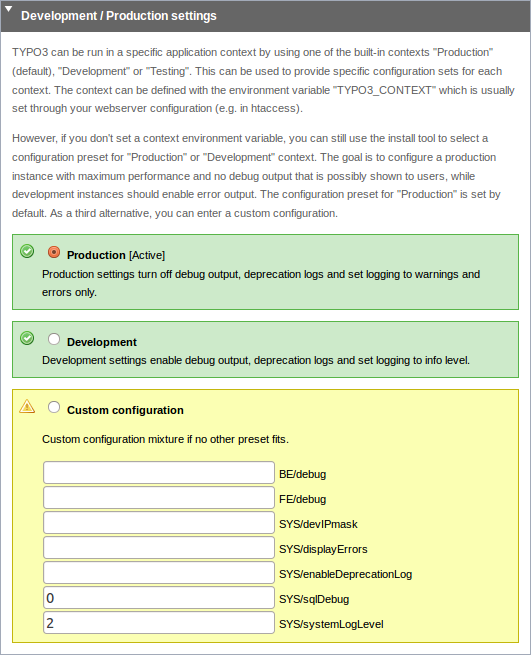
\includegraphics[width=0.8\linewidth]{Images/InstallTool/PresetsOfSettings.png}
			\end{figure}

		\end{column}
	\end{columns}

\end{frame}

% ------------------------------------------------------------------------------
% Improved Usability
% ------------------------------------------------------------------------------

\begin{frame}[fragile]
	\frametitle{Install Tool}
	\framesubtitle{Improved Usability}

	\begin{columns}[T]
		\begin{column}{.5\textwidth}

			\begin{itemize}
				\item Fixed position of menu left-\newline
					hand-side when scrolling
					\begingroup\color{typo3red}\textbf{(1)}\endgroup
				\item Fixed position of button "Write configuration" at the bottom
					\begingroup\color{typo3red}\textbf{(2)}\endgroup
				\item Entries in "All Configuration" are grouped (unfold a section by click on headline) and sorted
					\begingroup\color{typo3red}\textbf{(3)}\endgroup
			\end{itemize}

		\end{column}
		\begin{column}{.5\textwidth}

			\begin{figure}\vspace*{-0.4cm}
				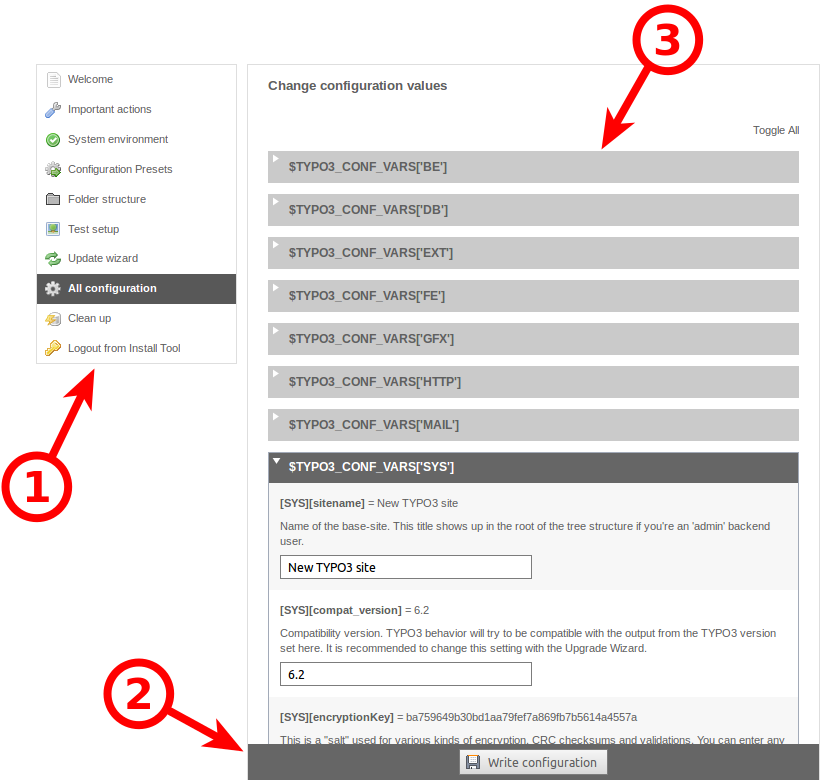
\includegraphics[width=0.8\linewidth]{Images/InstallTool/ImprovedUsability.png}
			\end{figure}

		\end{column}
	\end{columns}

\end{frame}

% ------------------------------------------------------------------------------
% Human-Friendly Error Codes
% ------------------------------------------------------------------------------

\begin{frame}[fragile]
	\frametitle{Install Tool}
	\framesubtitle{Human-Friendly Error Codes}

	\begin{itemize}
		\item Meaningful keywords can be used for the following options:\newline
			(TYPO3 < 6.2: numeric values only)
	\end{itemize}

	\begin{columns}[T]
		\begin{column}{.4\textwidth}
			\advance\leftskip+0.8cm

			\smaller
				\texttt{[SYS][errorHandlerErrors]}\newline
				\texttt{[SYS][exceptionalErrors]}\newline
				\texttt{[SYS][syslogErrorReporting]}\newline
				\texttt{[SYS][belogErrorReporting]}\newline
			\normalsize

		\end{column}
		\begin{column}{.6\textwidth}

			\begin{figure}\vspace*{-0.4cm}
				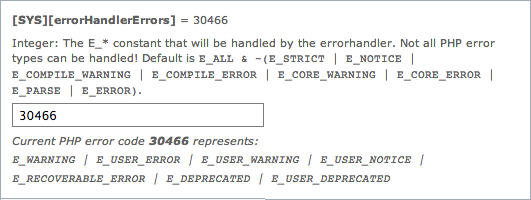
\includegraphics[width=0.9\linewidth]{Images/InstallTool/HumanFriendlyErrorCodes.png}
			\end{figure}

		\end{column}
	\end{columns}

	\vspace{0.2cm}

	\begin{itemize}
		\item An Extbase ViewHelper \textbf{format.phpErrorCode} takes care of the conversion to PHP error codes
	\end{itemize}

\end{frame}

% ------------------------------------------------------------------------------
% Errors In Folder Structure
% ------------------------------------------------------------------------------

\begin{frame}[fragile]
	\frametitle{Install Tool}
	\framesubtitle{Errors In Folder Structure}

	\begin{itemize}
		\item Errors under "Folder Structure" are listed as a badge (circled number)
	\end{itemize}

	\begin{figure}
		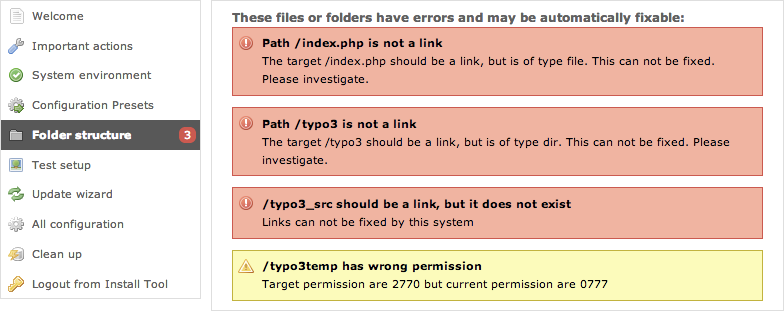
\includegraphics[width=0.95\linewidth]{Images/InstallTool/ErrorsInFolderStructure.png}
	\end{figure}

\end{frame}

% ------------------------------------------------------------------------------
% Core Updates
% ------------------------------------------------------------------------------

\begin{frame}[fragile]
	\frametitle{Install Tool}
	\framesubtitle{Core Updates}

	\begin{itemize}
		\item Update TYPO3 core to its latest minor version with a click of a button 
		\item Environment variable \texttt{TYPO3\_DISABLE\_CORE\_UPDATER=1} disables this feature
	\end{itemize}

	\begin{figure}
		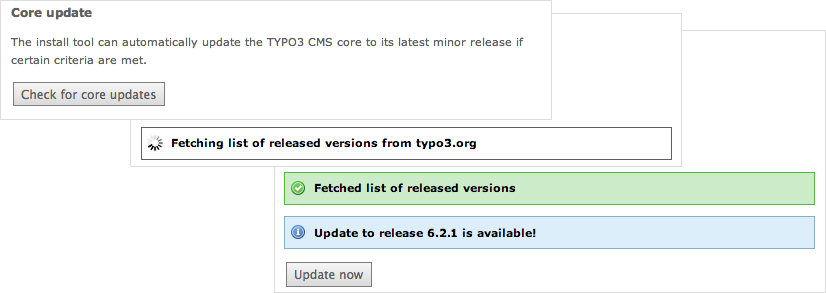
\includegraphics[width=0.95\linewidth]{Images/InstallTool/CoreUpdate.png}
	\end{figure}

\end{frame}

% ------------------------------------------------------------------------------
% Miscellaneous
% ------------------------------------------------------------------------------

\begin{frame}[fragile]
	\frametitle{Install Tool}
	\framesubtitle{Miscellaneous}

	\begin{itemize}
		\item All forms are CSRF (\textit{cross-site request forgery}) protected
		\item Install Tool uses a simplified Fluid Standalone View
		\item Only essential TYPO3 functions are loaded\newline
			(corrupt \texttt{ext\_localconf.php} or \texttt{ext\_tables.php} of extensions can not break the Install Tool any more)
		\item New starting point:	\tabto{3.2cm} \texttt{typo3/sysext/install/Start/Install.php}\newline
			Before:					\tabto{3.2cm} \texttt{typo3/install/index.php}\newline
									\tabto{3.2cm} (redirect from old to new URL exists)
		\item Deactivated cache ensures that Install Tool remains usable, even if cache contains invalid PHP code
	\end{itemize}

\end{frame}

% ------------------------------------------------------------------------------
% Miscellaneous
% ------------------------------------------------------------------------------

\begin{frame}[fragile]
	\frametitle{Install Tool}
	\framesubtitle{Miscellaneous}

	\begin{itemize}
		\item Check if PHP option \texttt{xdebug.max\_nesting\_level} shows a value of 250 or higher (default value "100" possibly causes problems)
		\item "Relaxed permission check":

			\small
				If the web root folder does not have correct permissions set (e.g. "2770"),
				and this issue can not be fixed, e.g. because the directory does not belong
				to the system user who runs the Install Tool, the first step of the installation
				breaks.
				The option "targetPermissionRelaxed" lowers the severity if permissions are not
				ideal and allows for continuing installation as long as required sub folders can
				be created.
			\normalsize

	\end{itemize}

\end{frame}

% ------------------------------------------------------------------------------
% Miscellaneous
% ------------------------------------------------------------------------------

\begin{frame}[fragile]
	\frametitle{Install Tool}
	\framesubtitle{Miscellaneous}

	\begin{itemize}
		\item Removed options (keys) from Install Tool\newline
			\small(and therefore from file \texttt{LocalConfiguration.php}, too):\normalsize
	\end{itemize}

	\begin{columns}[T]
		\begin{column}{.5\textwidth}
			\advance\leftskip+0.8cm
			\smaller
				\texttt{BE/loginLabels}\newline
				\texttt{BE/loginNews}\newline
				\texttt{BE/useOnContextMenuHandler}\newline
				\texttt{EXT/em\_mirrorListURL}\newline
				\texttt{EXT/em\_wsdlURL}\newline
				\texttt{EXT/extList}\newline
				\texttt{EXT/extList\_FE}\newline
				\texttt{EXT/noEdit}\newline
			\normalsize
		\end{column}
		\begin{column}{.5\textwidth}
			\smaller
				\texttt{FE/defaultTypoScript\_editorcfg}\newline
				\texttt{FE/simulateStaticDocuments}\newline
				\texttt{GFX/noIconProc}\newline
				\texttt{GFX/TTFLocaleConv}\newline
				\texttt{SYS/additionalAllowedClassPrefixes}\newline
				\texttt{SYS/caching/cacheBackends}\newline
				\texttt{SYS/caching/cacheFrontends}\newline
				\texttt{SYS/extCache}\newline
				\texttt{SYS/T3instID}\newline
			\normalsize
		\end{column}

	\end{columns}

\end{frame}

% ------------------------------------------------------------------------------



% ------------------------------------------------------------------------------
% Chapter 2: TYPO3 CMS Goes Responsive
% ------------------------------------------------------------------------------

% ------------------------------------------------------------------------------
% TYPO3 CMS 6.2 LTS - What's New - Chapter "Responsive Images" (French Version)
%
% @author	Paul Blondiaux <pblondiaux@sodifrance.fr>
% @author	Philippe Herault <philippe.herault@plan-net.fr>
% @license	Creative Commons BY-NC-SA 3.0
% @link		http://typo3.org/download/release-notes/whats-new/
% @language	French
% ------------------------------------------------------------------------------
% Chapter: Responsive Images
% ------------------------------------------------------------------------------

\section{Responsive Images}
\begin{frame}[fragile]
	\frametitle{Images « Responsive »}

	\begin{center}\huge{Chapitre 2 :}\end{center}
	\begin{center}\huge{\color{typo3darkgrey}\textbf{Images « Responsive »}}\end{center}

\end{frame}

% ------------------------------------------------------------------------------
% Select Screen Size In Page Preview
% ------------------------------------------------------------------------------

\begin{frame}[fragile]
	\frametitle{Images « Responsive »}
	\framesubtitle{Sélectionner une taille d'écran dans la prévisualisation de la page}

	\begin{itemize}
		\item Les contributeurs peuvent sélectionner différentes tailles d'écran dans le module « View » pour tester les sites « Responsive »
	\end{itemize}

	\begin{figure}
		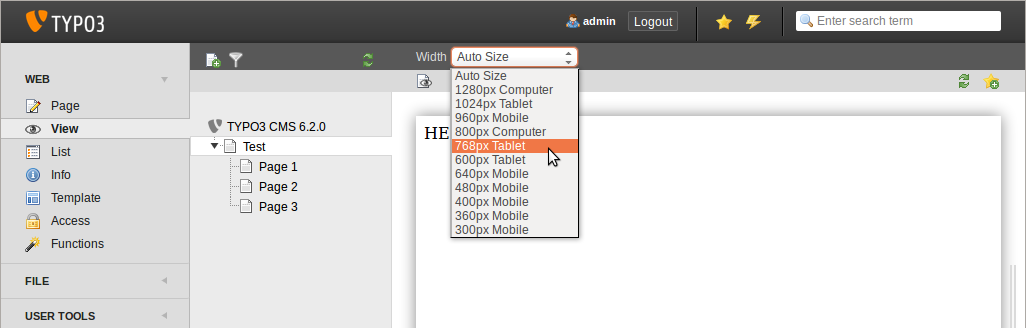
\includegraphics[width=0.95\linewidth]{Images/ResponsiveImages/ScreenSizeInPagePreview.png}
	\end{figure}

\end{frame}

% ------------------------------------------------------------------------------
% Customize Available Screen Sizes
% ------------------------------------------------------------------------------

\begin{frame}[fragile]
	\frametitle{Images « Responsive »}
	\framesubtitle{Personnaliser les tailles d'écran disponibles}

	\begin{itemize}
		\item Les tailles d'écran sont configurables en PageTSconfig :

		\lstset{
			basicstyle=\fontsize{7}{9}\selectfont\ttfamily
		}

		\begin{lstlisting}
			mod.web_view.previewFrameWidths {
			  1780.label = <any LLL or string>
			  1780.height = 145
			}
		\end{lstlisting}

		\item La largeur est définie par une variable (ici : 1780), la hauteur est optionnelle
		\item Des tailles prédéfinies sont disponibles dans :\newline
			\small\texttt{typo3/sysext/core/Configuration/DefaultConfiguration.php}\normalsize
		\item Les libellés peuvent être définis en PageTSconfig :

		\begin{lstlisting}
			mod.web_view.previewFrameWidths {
			  1280.label = LLL:EXT:viewpage/Resources/Private/Language/locallang.xlf:computer
			  1024.label = LLL:EXT:viewpage/Resources/Private/Language/locallang.xlf:tablet
			}
		\end{lstlisting}

	\end{itemize}

\end{frame}

% ------------------------------------------------------------------------------
% Responsive Image Galleries
% ------------------------------------------------------------------------------

\begin{frame}[fragile]
	\frametitle{Images « Responsive »}
	\framesubtitle{Galeries d'images « Responsive »}

	\begin{itemize}
		\item Attributs additionnels pour implémenter des galeries d'images « Responsive »
		\item L'extension « CSS styled content » a été enrichie
		\item Exemple: HTML5 (nécessite \texttt{config.doctype = html5})\newline

			TYPO3 CMS < 6.2:

			\lstset{
				basicstyle=\fontsize{7}{9}\selectfont\ttfamily
			}

			\begin{lstlisting}
				<div class="csc-textpic-imagewrap">...</div>
			\end{lstlisting}

			TYPO3 CMS >= 6.2:

			\begin{lstlisting}
				<div class="csc-textpic-imagewrap"
				  data-csc-images="{register:imageCount}"
				  data-csc-cols="{field:imagecols}">...</div>
			\end{lstlisting}

	\end{itemize}

\end{frame}

% ------------------------------------------------------------------------------
% Responsive Image Rendering
% ------------------------------------------------------------------------------

\begin{frame}[fragile]
	\frametitle{Images « Responsive »}
	\framesubtitle{Rendu des images « Responsive »}

	\begin{itemize}
		\item cObject IMAGE fournit un « sourceCollection » pour supporter diverses résolutions d'écran
		\item Le rendu des images pour les cObjects « texte/image » et « image » nécessite deux paramétrages dans l'éditeur de constantes :

			\texttt{styles.content.imgtext.responsive}\newline
			\texttt{styles.content.imgtext.layoutKey}

		\item Les options « clé en main » sont :

			\begin{itemize}
				\item \texttt{default} :	\tabto{2cm} balise \texttt{<img>} par défaut
				\item \texttt{srcset} :	\tabto{2cm} balise \texttt{<img>} avec les sources alternatives à l'aide de l'attribut \texttt{srcset}
				\item \texttt{picture} :	\tabto{2cm} balise \texttt{<picture>} avec les balises enfant \texttt{source}
				\item \texttt{data} :	\tabto{2cm} balise \texttt{<img>} avec les sources alternatives à l'aide d'attributs \texttt{data}
			\end{itemize}

	\end{itemize}

\end{frame}

% ------------------------------------------------------------------------------
% Property: layoutKey
% ------------------------------------------------------------------------------

\begin{frame}[fragile]
	\frametitle{Images « Responsive »}
	\framesubtitle{Propriété : layoutKey}

	\begin{itemize}
		\item \texttt{layoutKey} définit la disposition\newline
			(il s'agit du code HTML utilisé pour la balise \texttt{<img>})
		\item Chaque option présente un comportement unique pour le rendu HTML
		\item l'option \texttt{default} produit une balise \texttt{<img>} classique\newline
			(à utiliser si le frontend n'est pas « Responsive »)
		\item L'implémentation d'un gabarit « Responsive » nécessite plusieurs tailles d'images pour les différentes résolutions et tailles d'écran
		\item Selon le framework HTML, les capacités du navigateur et les bibliothèques JavaScript (pour une amélioration progressive) :

			\begin{itemize}
				\item utilisez un des gabarits préconfigurés ou
				\item définissez le vôtre
			\end{itemize}

	\end{itemize}

\end{frame}

% ------------------------------------------------------------------------------
% Property: layout
% ------------------------------------------------------------------------------

\begin{frame}[fragile]
	\frametitle{Images « Responsive »}
	\framesubtitle{Propriété : layout}

	\lstset{
		basicstyle=\tiny\ttfamily
	}

	\begin{lstlisting}
		layoutKey = {$styles.content.imgtext.layoutKey}
		layout {
		  default {
		    element = <img src="###SRC###" width="###WIDTH###" height="###HEIGHT###" ###PARAMS###
		      ###ALTPARAMS### ###BORDER######SELFCLOSINGTAGSLASH###>
		  }
		  srcset {
		    element = <img src="###SRC###" srcset="###SOURCECOLLECTION###" ###PARAMS###
		      ###ALTPARAMS### ###SELFCLOSINGTAGSLASH###>
		    source = |*|###SRC### ###SRCSETCANDIDATE###,|*|###SRC### ###SRCSETCANDIDATE###
		  }
		  picture {
		    element = <picture>###SOURCECOLLECTION###<img src="###SRC###" ###PARAMS###
		      ###ALTPARAMS######SELFCLOSINGTAGSLASH###></picture>
		    source = <source src="###SRC###" media="###MEDIAQUERY###"###SELFCLOSINGTAGSLASH###>
		  }
		  data {
		    element = <img src="###SRC###" ###SOURCECOLLECTION### ###PARAMS###
		      ###ALTPARAMS######SELFCLOSINGTAGSLASH###>
		    source = data-###DATAKEY###="###SRC###"
		  }
		}
	\end{lstlisting}

\end{frame}

% ------------------------------------------------------------------------------
% Property: layout.[layoutKey].element
% ------------------------------------------------------------------------------

\begin{frame}[fragile]
	\frametitle{Images « Responsive »}
	\framesubtitle{Propriété : layout.[layoutKey].element}

	\begin{itemize}
		\item \lstinline!###SRC###!\newline
			URL pour l'attribut : \texttt{src}

		\item \lstinline!###WIDTH###!\newline
			Largeur (en pixel) pour l'attribut : \texttt{width}

		\item \lstinline!###HEIGHT###!\newline
			Hauteur (en pixel) pour l'attribut : \texttt{height}

		\item \lstinline!###PARAMS###!\newline
			Paramètres additionnels tels que définis dans le cObject « IMAGE »

		\item \lstinline!###ALTPARAMS###!\newline
			Paramètres additionnels alternatifs tels que définis dans le cObject « IMAGE »
	\end{itemize}

\end{frame}

% ------------------------------------------------------------------------------
% Property: layout.[layoutKey].element
% ------------------------------------------------------------------------------

\begin{frame}[fragile]
	\frametitle{Images « Responsive »}
	\framesubtitle{Propriété : layout.[layoutKey].element}

	\begin{itemize}
		\item \lstinline!###BORDER###!\newline
			Bordure (en pixel) pour l'attribut : \texttt{border}

		\item \lstinline!###SELFCLOSINGTAGSLASH###!\newline
			Balise fermante, par exemple : \texttt{<img ... />} vs. \texttt{<img ... >}\newline
			(dépend de \texttt{config.xhtmlDoctype} ou de \texttt{config.doctype})

		\item \lstinline!###SOURCECOLLECTION###!\newline
			Images sources additionnelles, dépend du design web « Responsive » utilisé.
			Les valeurs exactes sont définies dans : \texttt{layout.[layoutKey].source}
	\end{itemize}

\end{frame}

% ------------------------------------------------------------------------------
% Property: sourceCollection.[dataKey]
% ------------------------------------------------------------------------------

\begin{frame}[fragile]
	\frametitle{Images « Responsive »}
	\framesubtitle{Propriété : sourceCollection.[dataKey]}

	\begin{itemize}
		\item « sourceCollection » par défaut de EXT:css\_styled\_content
		\item Créer votre propre « sourceCollection » est vivement recommandé

			\lstset{
				basicstyle=\tiny\ttfamily
			}

			\begin{lstlisting}
				sourceCollection {
				  small {
				    width = 200
				    srcsetCandidate = 600w
				    mediaQuery = (max-device-width: 600px)
				    dataKey = small
				  }
				  smallRetina {
				    if.directReturn = 1
				    width = 200
				    pixelDensity = 2
				    srcsetCandidate = 600w 2x
				    mediaQuery = (max-device-width: 600px) AND (min-resolution: 192dpi)
				    dataKey = smallRetina
				  }
				}
			\end{lstlisting}
	\end{itemize}

\end{frame}

% ------------------------------------------------------------------------------
% Further Resources (External Links)
% ------------------------------------------------------------------------------

\begin{frame}[fragile]
	\frametitle{Images « Responsive »}
	\framesubtitle{Aller plus loin}

	\begin{itemize}
		\item Exemple de code fonctionnel :\newline
			\small\url{http://wiki.typo3.org/Responsive_Image_Rendering}\normalsize

		\item Article de Sven Wolfermann sur typo3.org :\newline
			\small\url{http://typo3.org/news/article/responsive-image-rendering-in-typo3-cms-62/}\normalsize

		\item Spécifications du W3C :\newline
			\small\url{http://www.w3.org/html/wg/drafts/srcset/w3c-srcset/}\newline
			\small\url{http://www.w3.org/TR/html-picture-element/}\normalsize

		\item Brouillon fonctionnel du « Responsive Image Community Group » :\newline
			\small\url{http://responsiveimages.org}\normalsize

	\end{itemize}

\end{frame}

% ------------------------------------------------------------------------------



% ------------------------------------------------------------------------------
% Chapter 3: Backend Changes
% ------------------------------------------------------------------------------

% ------------------------------------------------------------------------------
% TYPO3 CMS 6.2 LTS - What's New - Chapter "Backend Changes" (English Version)
%
% @author	Michael Schams <schams.net>
% @license	Creative Commons BY-NC-SA 3.0
% @link		http://typo3.org/download/release-notes/whats-new/
% @language	English
% ------------------------------------------------------------------------------
% Chapter: Backend Changes
% ------------------------------------------------------------------------------

\section{Backend Changes}
\begin{frame}[fragile]
	\frametitle{Backend Changes}

	\begin{center}\huge{Chapter 3:}\end{center}
	\begin{center}\huge{\color{typo3darkgrey}\textbf{Backend Changes}}\end{center}

\end{frame}

% ------------------------------------------------------------------------------
% Autofocus
% ------------------------------------------------------------------------------
% http://forge.typo3.org/issues/49228

\begin{frame}[fragile]
	\frametitle{Backend Changes}
	\framesubtitle{Backend Login}

 	\begin{itemize}
		\item Autofocus on username field in the backend login form\newline
			(HTML5 attribute: \texttt{autofocus="autofocus"})
	\end{itemize}

	\begin{figure}
		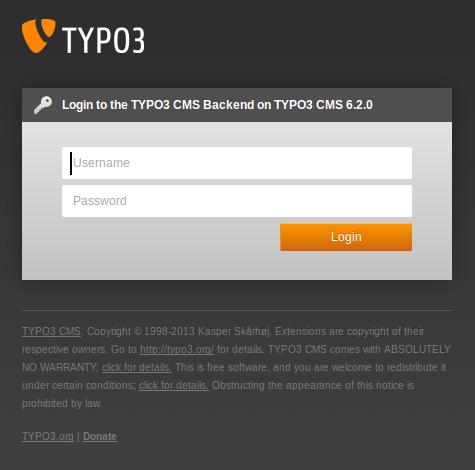
\includegraphics[width=0.4\linewidth]{Images/BackendChanges/BackendLogin.png}
	\end{figure}

\end{frame}

% ------------------------------------------------------------------------------
% Visual Appearance
% ------------------------------------------------------------------------------
% http://forge.typo3.org/issues/48376

\begin{frame}[fragile]
	\frametitle{Backend Changes}
	\framesubtitle{Visual Appearance}

	\begin{columns}[T]

		\begin{column}{.5\textwidth}
			\begin{itemize}
				\item Improved usability by livening the layout up
				\item Margins between module items (left-hand-side column) increased
				\item Based on a 12px grid, which has been doubled
			\end{itemize}

			\advance\leftskip+3.8cm

			\smaller
				Left: TYPO3 4.5\newline
				Right: TYPO3 6.2
			\normalsize
		\end{column}

		\begin{column}{.5\textwidth}
			\begin{figure}\vspace*{-0.4cm}
				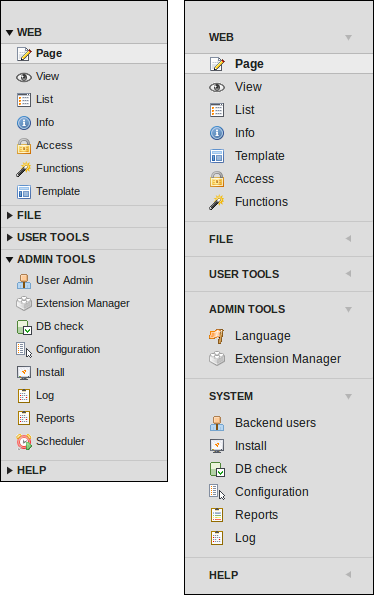
\includegraphics[width=0.6\linewidth]{Images/BackendChanges/VisualAppearance.png}
			\end{figure}
		\end{column}

	\end{columns}

\end{frame}

% ------------------------------------------------------------------------------
% Visual Appearance
% ------------------------------------------------------------------------------

\begin{frame}[fragile]
	\frametitle{Backend Changes}
	\framesubtitle{Visual Appearance}

	\begin{columns}[T]

		\begin{column}{.5\textwidth}

			\begin{itemize}
				\item Modules in left-hand-side column restructured
				\item Module "ADMINTOOLS" divided into two parts:

					\begin{itemize}
						\item \textbf{ADMINTOOLS} ("Languages" and "Extension Manager")
						\item \textbf{SYSTEM} (low-level tools, which do not show the page tree column)
					\end{itemize}

				\item Module "TypoScript Help" removed (obsolete)

			\end{itemize}

		\end{column}

		\begin{column}{.5\textwidth}
			\begin{figure}\vspace*{-0.4cm}
				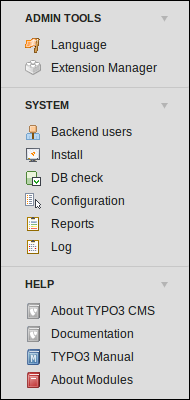
\includegraphics[width=0.35\linewidth]{Images/BackendChanges/AdminTools.png}
			\end{figure}
		\end{column}

	\end{columns}

\end{frame}

% ------------------------------------------------------------------------------
% Visual Appearance
% ------------------------------------------------------------------------------
% http://forge.typo3.org/issues/36017

\begin{frame}[fragile]
	\frametitle{Backend Changes}
	\framesubtitle{Visual Appearance}

	\begin{itemize}
		\item \texttt{<h1>}-headlines in main area use TYPO3 font "Share" consistantly
	\end{itemize}

	\begin{figure}
		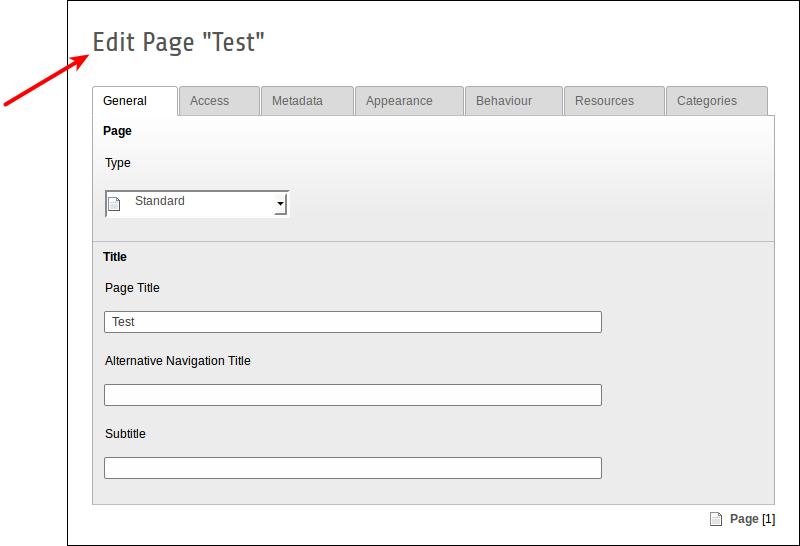
\includegraphics[width=0.6\linewidth]{Images/BackendChanges/ConsistantFont.png}
	\end{figure}

\end{frame}

% ------------------------------------------------------------------------------
% Visual Appearance
% ------------------------------------------------------------------------------
% http://forge.typo3.org/issues/41631

\begin{frame}[fragile]
	\frametitle{Backend Changes}
	\framesubtitle{Visual Appearance}

	\begin{itemize}
		\item Module "Reports" shows new icon
	\end{itemize}

	\begin{figure}
		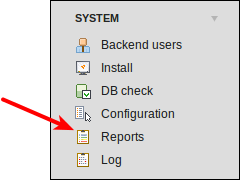
\includegraphics[width=0.35\linewidth]{Images/BackendChanges/ModuleReportsIcon.png}
	\end{figure}

\end{frame}

% ------------------------------------------------------------------------------
% Drag&Drop File Upload in Filelist (FAL)
% ------------------------------------------------------------------------------
% http://forge.typo3.org/issues/47005

\begin{frame}[fragile]
	\frametitle{Backend Changes}
	\framesubtitle{Drag\&Drop File Upload (1)}

	\begin{itemize}
		\item HTML5 Drag\&Drop file upload functionality implemented in filelist

	\end{itemize}

	\begin{figure}
		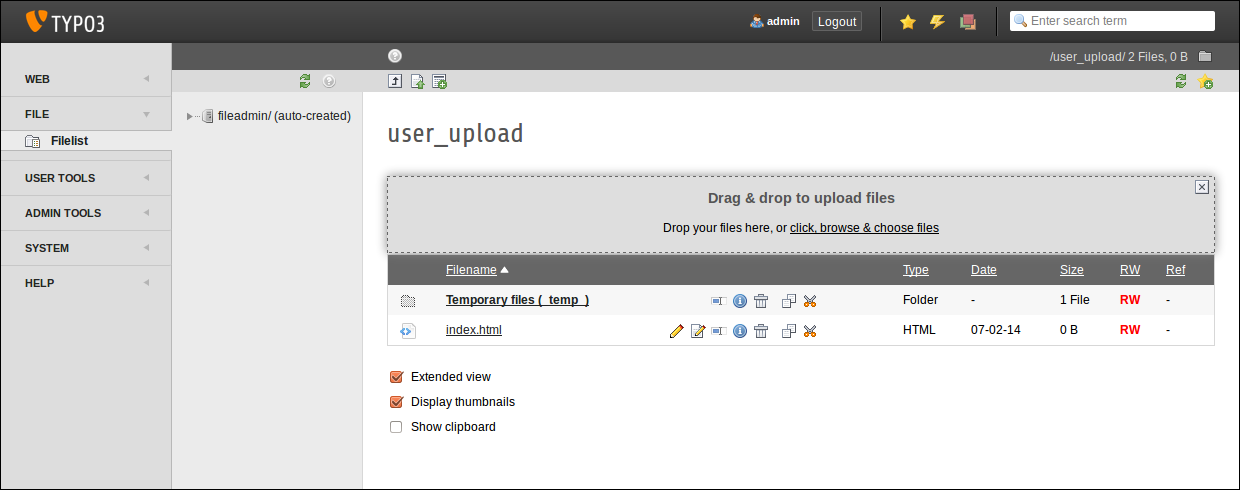
\includegraphics[width=0.95\linewidth]{Images/BackendChanges/DragDropFileUpload.png}
	\end{figure}

\end{frame}

% ------------------------------------------------------------------------------
% Drag&Drop File Upload Via Content Elements
% (slide added in March 2014)
% ------------------------------------------------------------------------------

\begin{frame}[fragile]
	\frametitle{Backend Changes}
	\framesubtitle{Drag\&Drop File Upload (2)}

	\begin{itemize}
		\item ...and via content elements (button: "Select \& upload files")

	\end{itemize}

	\begin{figure}
		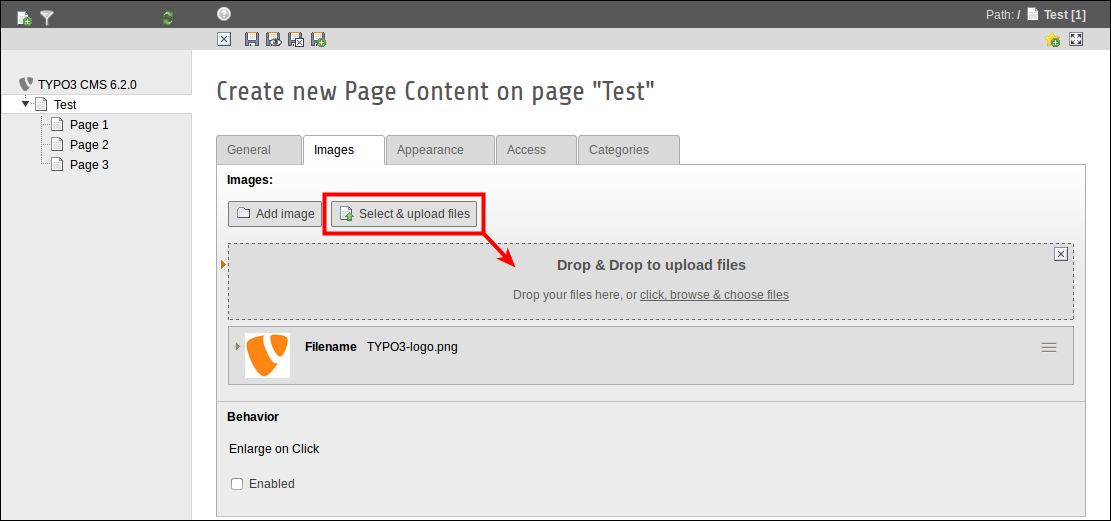
\includegraphics[width=0.95\linewidth]{Images/BackendChanges/SelectAndUploadFiles.png}
	\end{figure}

\end{frame}

% ------------------------------------------------------------------------------
% Backend Users
% ------------------------------------------------------------------------------
% http://forge.typo3.org/issues/43053

\begin{frame}[fragile]
	\frametitle{Backend Changes}
	\framesubtitle{Usability: Backend User List}

	\begin{itemize}
		\item Username and real name is shown (first column in list view)
		\item Click on (user)name links to edit user record
		\item Delete button added to list view

	\end{itemize}

	\begin{figure}
		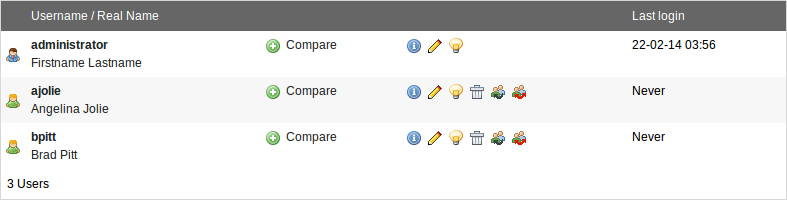
\includegraphics[width=0.95\linewidth]{Images/BackendChanges/BackendUserList.png}
	\end{figure}

\end{frame}

% ------------------------------------------------------------------------------
% Live Search
% ------------------------------------------------------------------------------
% http://forge.typo3.org/issues/35358

\begin{frame}[fragile]
	\frametitle{Backend Changes}
	\framesubtitle{Live Search}

	\begin{itemize}
		\item Tooltip shows UID as well as PID in "livesearch"
		\item When, after a search, the edit form is closed again, the list view of the page is shown (not an empty page)
	\end{itemize}

	\begin{figure}
		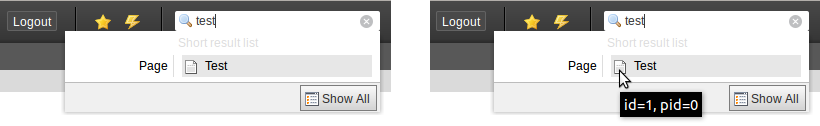
\includegraphics[width=0.8\linewidth]{Images/BackendChanges/LiveSearchTooltip.png}
	\end{figure}

\end{frame}

% ------------------------------------------------------------------------------
% Live Search
% ------------------------------------------------------------------------------

\begin{frame}[fragile]
	\frametitle{Backend Changes}
	\framesubtitle{Live Search}

	\begin{itemize}
		\item In TYPO3 < 6.2, for pages, only database fields \texttt{title} and \texttt{uid} are taken into account
		\item In TYPO3 >= 6.2, field \texttt{alias} can be added to search\newline
			(requires UserTSconfig: \texttt{options.pageTree.searchInAlias = 1})
	\end{itemize}

	\begin{figure}
		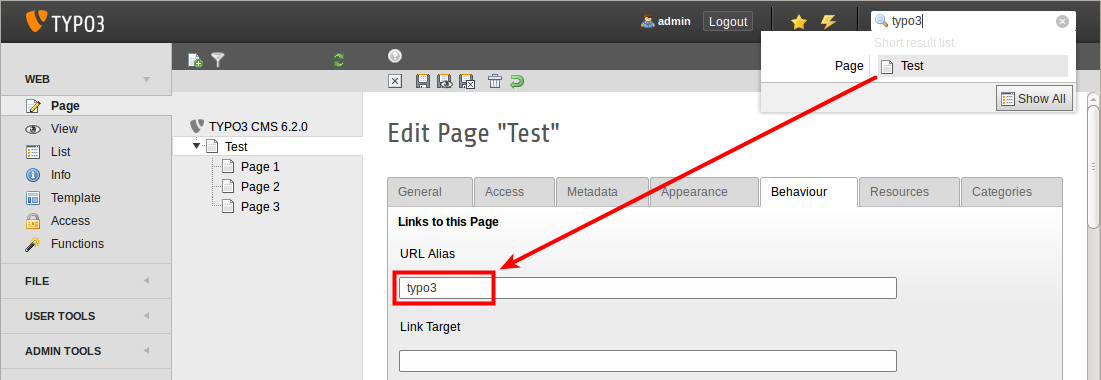
\includegraphics[width=0.95\linewidth]{Images/BackendChanges/LiveSearchInAlias.png}
	\end{figure}

\end{frame}

% ------------------------------------------------------------------------------
% File Abstraction Layer
% ------------------------------------------------------------------------------

\begin{frame}[fragile]
	\frametitle{Backend Changes}
	\framesubtitle{File Abstraction Layer}

	\begin{itemize}
		\item Title and filename are shown in FAL element header
	\end{itemize}

	\begin{figure}
		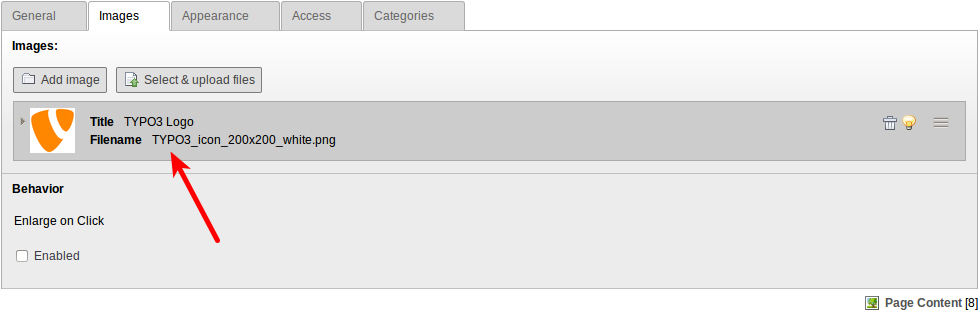
\includegraphics[width=0.95\linewidth]{Images/BackendChanges/FalTitleAndFilename.png}
	\end{figure}

\end{frame}

% ------------------------------------------------------------------------------
% File Abstraction Layer
% ------------------------------------------------------------------------------

\begin{frame}[fragile]
	\frametitle{Backend Changes}
	\framesubtitle{File Abstraction Layer (EXT:filemetadata)}

	\begin{itemize}
		\item System extension "filemetadata" add tabs to show meta data\newline
			\small(extension is shipped with the core, but not installed by default)\normalsize
	\end{itemize}

	\begin{figure}
		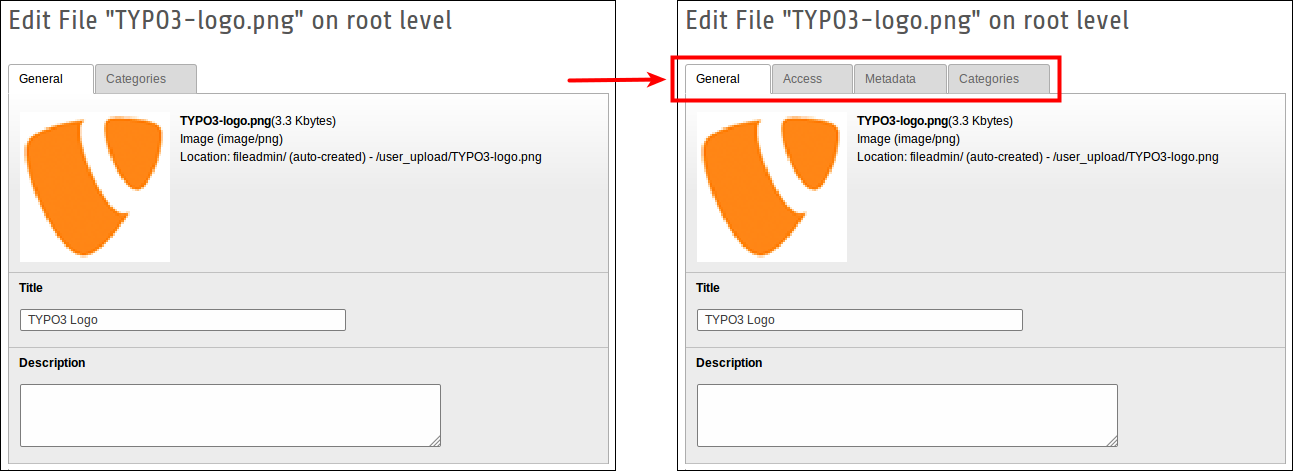
\includegraphics[width=0.95\linewidth]{Images/BackendChanges/FileMetaDataTabs.png}
	\end{figure}

\end{frame}

% ------------------------------------------------------------------------------
% File Abstraction Layer
% ------------------------------------------------------------------------------

\begin{frame}[fragile]
	\frametitle{Backend Changes}
	\framesubtitle{File Abstraction Layer (EXT:filemetadata)}

	\begin{figure}
		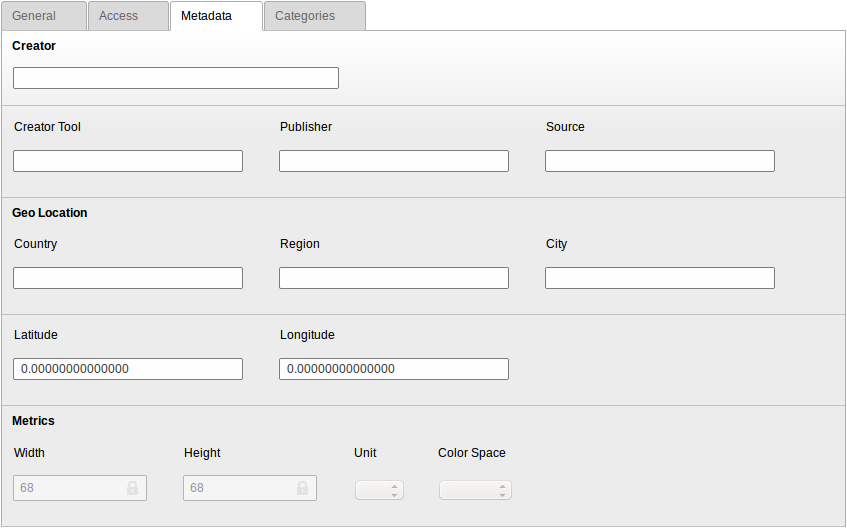
\includegraphics[width=0.8\linewidth]{Images/BackendChanges/FileMetaData.png}
	\end{figure}

\end{frame}

% ------------------------------------------------------------------------------
% File Abstraction Layer
% ------------------------------------------------------------------------------

\begin{frame}[fragile]
	\frametitle{Backend Changes}
	\framesubtitle{File Abstraction Layer}

	\begin{itemize}
		\item It is now possible to translate FAL meta data into frontend languages
	\end{itemize}

	\begin{figure}
		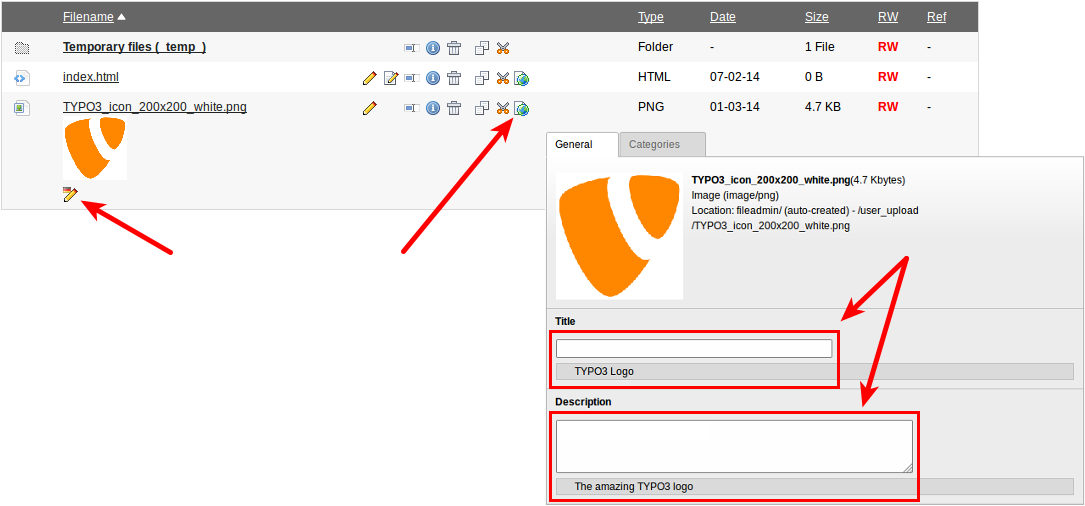
\includegraphics[width=0.95\linewidth]{Images/BackendChanges/FalTranslateMetaData.png}
	\end{figure}

\end{frame}

% ------------------------------------------------------------------------------
% Module: Documentation
% ------------------------------------------------------------------------------

\begin{frame}[fragile]
	\frametitle{Backend Changes}
	\framesubtitle{Module: Documentation}

	\begin{columns}[T]

		\begin{column}{.5\textwidth}
			\begin{itemize}
				\item Module "Documentation" allows BE users to download and view manuals
				\item New TYPO3 installations load this module by default
				\item Function "Download Documentation" downloads manuals (see illustration)
				\item Use the Extension Manager to load "Documentation" in an updated TYPO3 installation
			\end{itemize}
		\end{column}

		\begin{column}{.5\textwidth}
			\begin{figure}\vspace*{-0.4cm}
				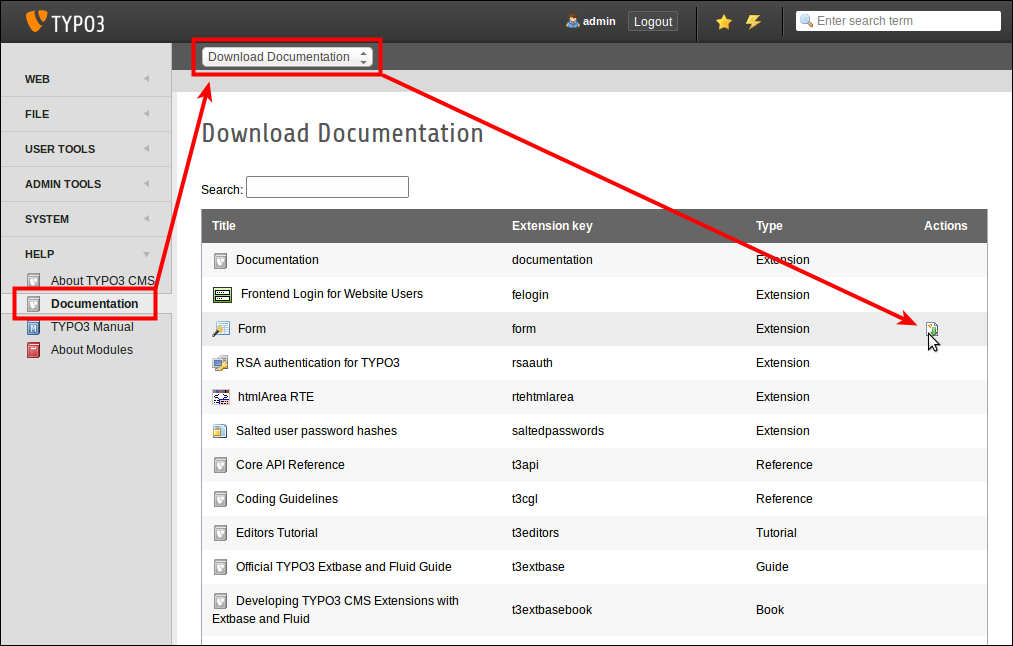
\includegraphics[width=1\linewidth]{Images/BackendChanges/DownloadDocumentation.png}
			\end{figure}
		\end{column}

	\end{columns}

\end{frame}

% ------------------------------------------------------------------------------
% Module: Documentation
% ------------------------------------------------------------------------------

\begin{frame}[fragile]
	\frametitle{Backend Changes}
	\framesubtitle{Module: Documentation}

	\begin{itemize}
		\item Function "Show Documentation" displays downloaded manuals
	\end{itemize}

	\begin{figure}
		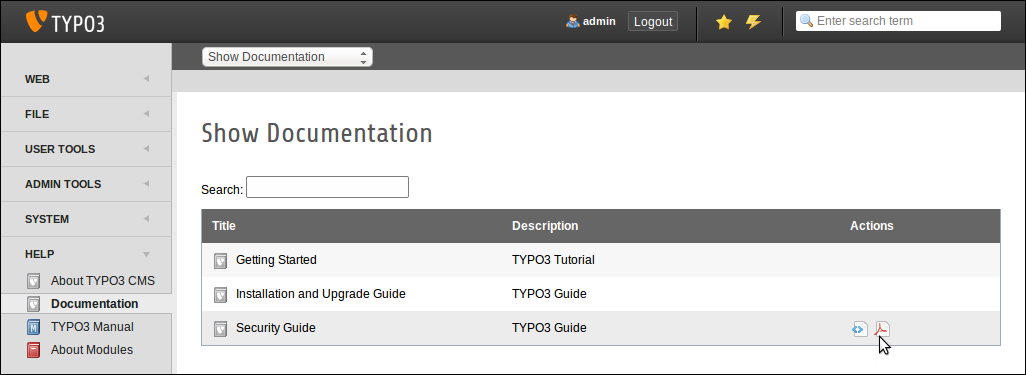
\includegraphics[width=0.95\linewidth]{Images/BackendChanges/ShowDocumentation.png}
	\end{figure}

\end{frame}

% ------------------------------------------------------------------------------
% Removed: TypoScript Help
% ------------------------------------------------------------------------------
% http://forge.typo3.org/issues/47931

\begin{frame}[fragile]
	\frametitle{Backend Changes}
	\framesubtitle{Removed: TypoScript Help}

 	\begin{itemize}
		\item EXT:tsconfig\_help ("TSconfig Quick Reference") removed\newline
			\small(outdated information and not maintained since TYPO3 CMS 4.1)
	\end{itemize}

	\begin{figure}
		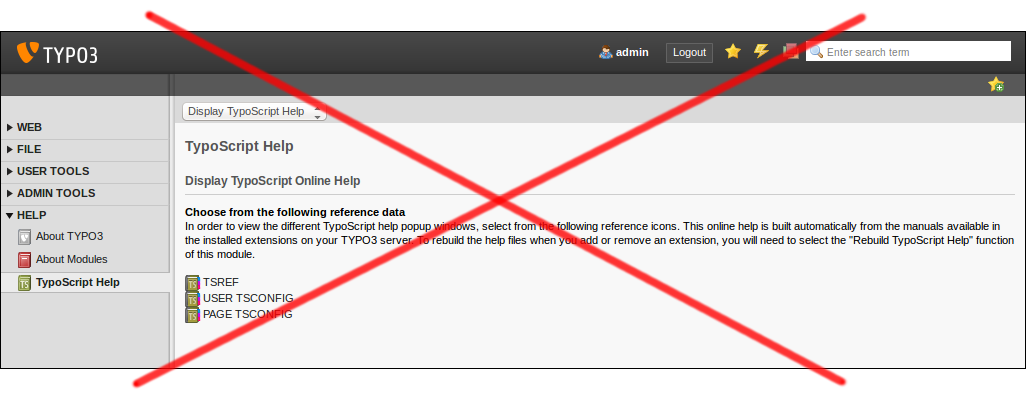
\includegraphics[width=0.95\linewidth]{Images/BackendChanges/TypoScriptHelpRemovedCrossed.png}
	\end{figure}

\end{frame}


% ------------------------------------------------------------------------------
% Scheduler
% ------------------------------------------------------------------------------

\begin{frame}[fragile]
	\frametitle{Backend Changes}
	\framesubtitle{Scheduler}

	\begin{itemize}
		\item Delete scheduler task in edit view\newline
			\small(in TYPO3 < 6.2, delete function was available in the list view only)\normalsize
	\end{itemize}

	\begin{figure}
		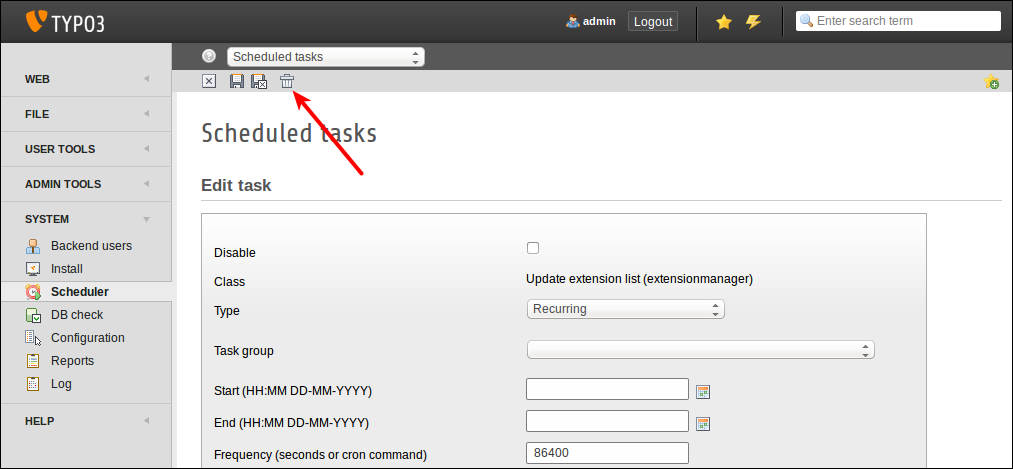
\includegraphics[width=0.95\linewidth]{Images/BackendChanges/DeleteSchedulerTaskInEditView.png}
	\end{figure}

\end{frame}

% ------------------------------------------------------------------------------
% Scheduler
% ------------------------------------------------------------------------------

\begin{frame}[fragile]
	\frametitle{Backend Changes}
	\framesubtitle{Scheduler}

	\begin{itemize}
		\item Description can be assigned to scheduler tasks and shown as subheaders in list view, or as tooltips (see next slide)
	\end{itemize}

	\begin{figure}
		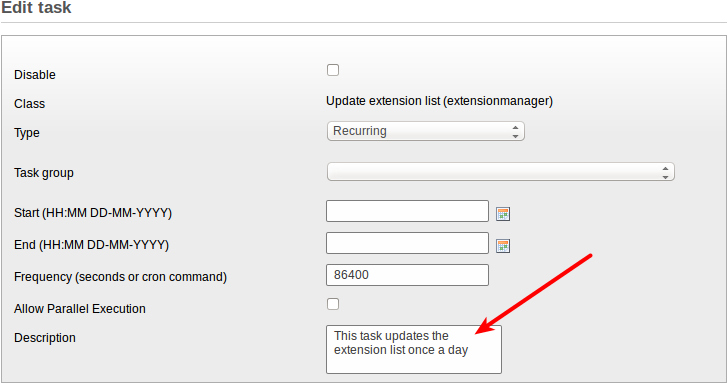
\includegraphics[width=0.7\linewidth]{Images/BackendChanges/SchedulerTaskDescription.png}
	\end{figure}

\end{frame}

% ------------------------------------------------------------------------------
% Scheduler
% ------------------------------------------------------------------------------

\begin{frame}[fragile]
	\frametitle{Backend Changes}
	\framesubtitle{Scheduler}

	\begin{itemize}
		\item Task description as subheader\newline
			\small(this features needs to be activated in extension configuration)\normalsize
	\end{itemize}

	\begin{figure}
		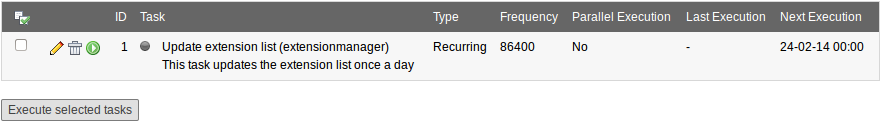
\includegraphics[width=0.95\linewidth]{Images/BackendChanges/SchedulerTaskDescriptionAsSubheader.png}
	\end{figure}

	\begin{itemize}
		\item Task description as tooltip ("hover")
	\end{itemize}

	\begin{figure}
		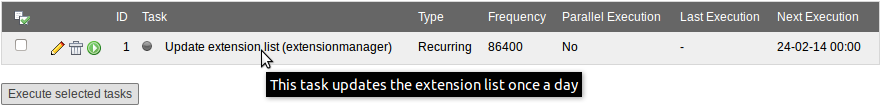
\includegraphics[width=0.95\linewidth]{Images/BackendChanges/SchedulerTaskDescriptionAsTooltip.png}
	\end{figure}

\end{frame}

% ------------------------------------------------------------------------------
% Scheduler
% ------------------------------------------------------------------------------

\begin{frame}[fragile]
	\frametitle{Backend Changes}
	\framesubtitle{Scheduler}

	\begin{itemize}
		\item It is now possible to group scheduler tasks
		\item Add "scheduler task group" records to root page (UID: 0)\newline
			and select group in the task
	\end{itemize}

	\begin{figure}
		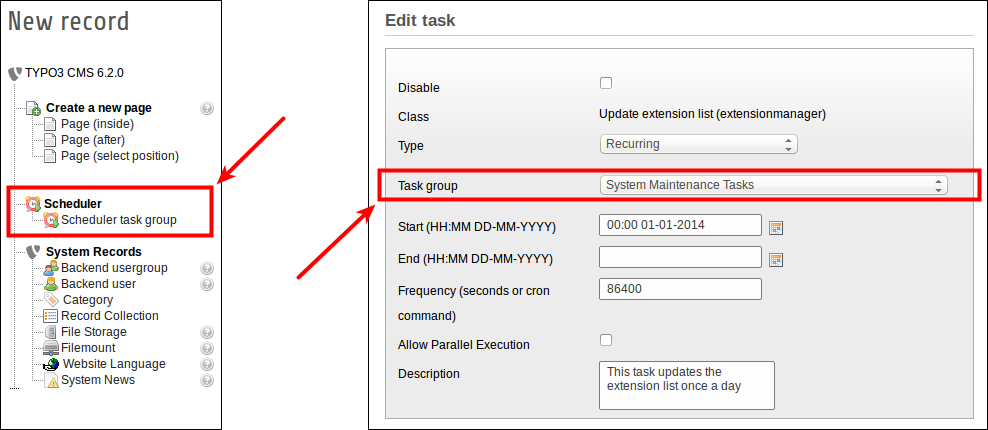
\includegraphics[width=0.85\linewidth]{Images/BackendChanges/SchedulerTaskGroup.png}
	\end{figure}

\end{frame}

% ------------------------------------------------------------------------------
% System Extension: Form
% ------------------------------------------------------------------------------
% http://forge.typo3.org/issues/38094

\begin{frame}[fragile]
	\frametitle{Backend Changes}
	\framesubtitle{System Extension: Form}

	\begin{columns}[T]

		\begin{column}{.5\textwidth}
			\begin{itemize}
				\item New post-processor for cObject FORM: \textbf{redirect}\newline
					(redirect after form submission)
				\item Value is parsed by \texttt{typolink} (TypoScript function),\newline
					which means, value can be a page ID or a URL
			\end{itemize}
		\end{column}

		\begin{column}{.5\textwidth}
			\begin{figure}\vspace*{-0.4cm}
				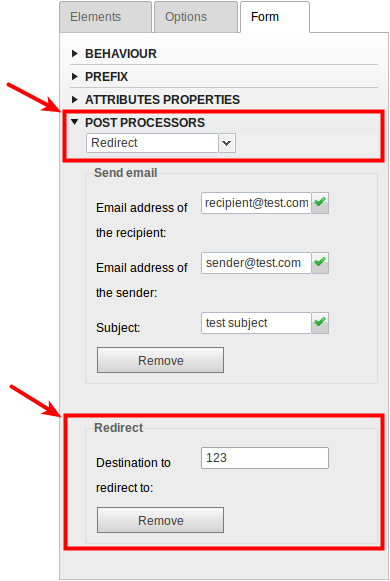
\includegraphics[width=0.65\linewidth]{Images/BackendChanges/FormRedirectPostProcessor.png}
			\end{figure}
		\end{column}

	\end{columns}

\end{frame}

% ------------------------------------------------------------------------------
% Module: List
% ------------------------------------------------------------------------------
% http://forge.typo3.org/issues/49810

\begin{frame}[fragile]
	\frametitle{Backend Changes}
	\framesubtitle{List Module}

	\begin{itemize}
		\item Additional columns "UID" and "PID" in list view for non-admins
	\end{itemize}

	\begin{figure}
		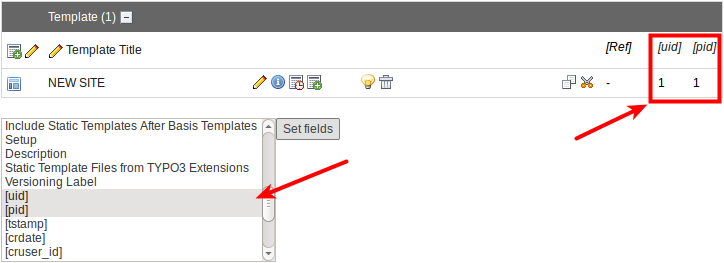
\includegraphics[width=0.95\linewidth]{Images/BackendChanges/AdditionalColumnsInListModule.png}
	\end{figure}

\end{frame}

% ------------------------------------------------------------------------------
% File Abstraction Layer
% ------------------------------------------------------------------------------
% http://forge.typo3.org/issues/50827
% http://forge.typo3.org/issues/51097

\begin{frame}[fragile]
	\frametitle{Backend Changes}
	\framesubtitle{File Abstraction Layer}

	\begin{itemize}
		\item If indexer detects a missing file, a message is shown and a flag in the database record is set
		\item Module "Reports" also lists this as an issue
		\item When file re-appears, message and flag are reset
	\end{itemize}

	\begin{columns}[T]

		\begin{column}{.5\textwidth}
			\begin{figure}
				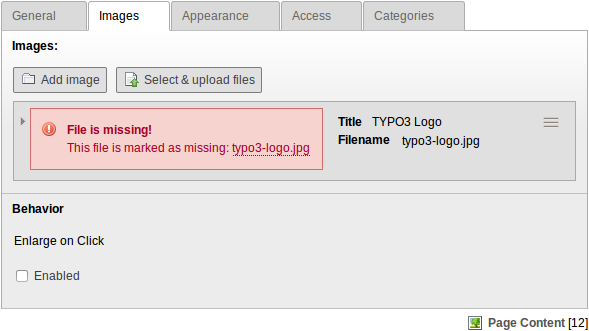
\includegraphics[width=0.95\linewidth]{Images/BackendChanges/FalMissingFileContentElement.png}
			\end{figure}
		\end{column}

		\begin{column}{.5\textwidth}
			\begin{figure}
				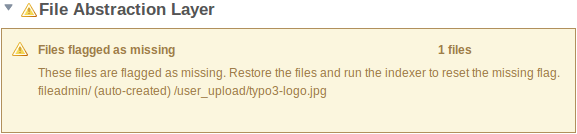
\includegraphics[width=0.95\linewidth]{Images/BackendChanges/FalMissingFileReportsModule.png}
			\end{figure}
		\end{column}

	\end{columns}

\end{frame}

% ------------------------------------------------------------------------------
% Menu/Sitemap: Category-based Menus
% ------------------------------------------------------------------------------
% http://forge.typo3.org/issues/51161

\begin{frame}[fragile]
	\frametitle{Backend Changes}
	\framesubtitle{Category-based Menus (1)}

	\begin{itemize}
		\item Content element "Menu/Sitemap" can create a menu, based on categories
	\end{itemize}

	\begin{figure}
		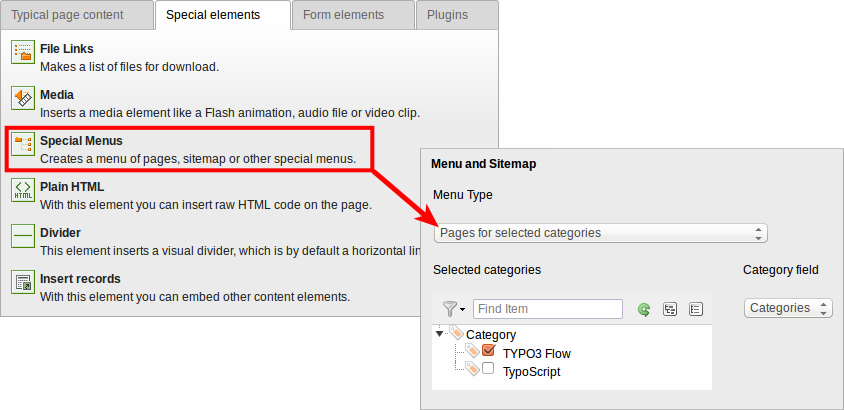
\includegraphics[width=0.8\linewidth]{Images/BackendChanges/CategoryBasedMenus.png}
	\end{figure}

\end{frame}

% ------------------------------------------------------------------------------
% Menu/Sitemap: Category-based Menus
% (slide added in March 2014)
% ------------------------------------------------------------------------------

\begin{frame}[fragile]
	\frametitle{Backend Changes}
	\framesubtitle{Category-based Menus (2)}

	\begin{itemize}
		\item Another new type of menu: "\underline{Content elements} for selected categories"
	\end{itemize}

	\begin{figure}
		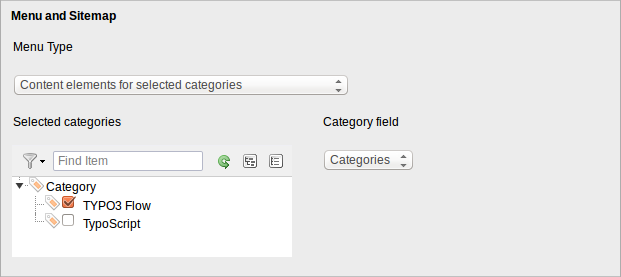
\includegraphics[width=0.6\linewidth]{Images/BackendChanges/ContentElementsForSelectedCategories.png}
	\end{figure}

\end{frame}

% ------------------------------------------------------------------------------
% Sorting Categories
% ------------------------------------------------------------------------------
% http://forge.typo3.org/issues/51590

\begin{frame}[fragile]
	\frametitle{Backend Changes}
	\framesubtitle{Sorting Categories}

 	\begin{itemize}
		\item Categories can be sorted now\newline
			\small(in TYPO3 < 6.2, categories are always sorted alphabetically)\normalsize
	\end{itemize}

	\begin{figure}
		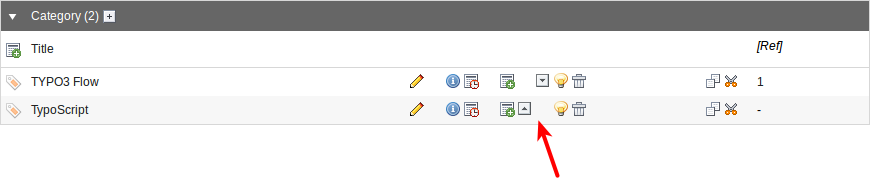
\includegraphics[width=0.95\linewidth]{Images/BackendChanges/CategorySorting.png}
	\end{figure}

\end{frame}

% ------------------------------------------------------------------------------
% Category Visibility
% ------------------------------------------------------------------------------
% http://forge.typo3.org/issues/52718

\begin{frame}[fragile]
	\frametitle{Backend Changes}
	\framesubtitle{Category Visibility}

 	\begin{itemize}
		\item Visibility of categories can be restricted for BE users/groups
	\end{itemize}

	\begin{figure}
		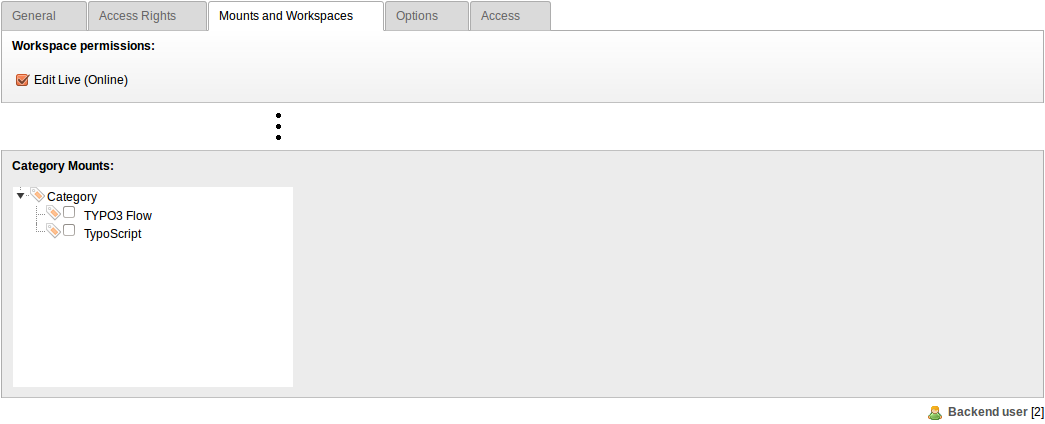
\includegraphics[width=0.95\linewidth]{Images/BackendChanges/CategoryVisibility.png}
	\end{figure}

\end{frame}

% ------------------------------------------------------------------------------
% "New Content" icon always visible
% ------------------------------------------------------------------------------
% http://forge.typo3.org/issues/48938
% http://forge.typo3.org/issues/51480

\begin{frame}[fragile]
	\frametitle{Backend Changes}
	\framesubtitle{Usability}

 	\begin{itemize}
		\item Icon "new content" is always visible if the column is empty\newline
			\small(this helps editors to understand what they can do)\normalsize
	\end{itemize}

	\begin{figure}
		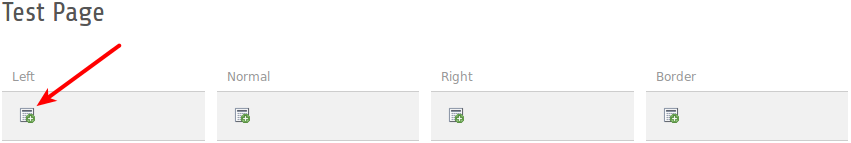
\includegraphics[width=0.95\linewidth]{Images/BackendChanges/NewContentIconAlwaysVisible.png}
	\end{figure}

\end{frame}

% ------------------------------------------------------------------------------
% Module "Functions": Hide In Menus
% ------------------------------------------------------------------------------
% http://forge.typo3.org/issues/51017

\begin{frame}[fragile]
	\frametitle{Backend Changes}
	\framesubtitle{Functions}

 	\begin{itemize}
		\item When creating multiple pages in module "functions", a new checkbox allows editors to hide these pages in menus\newline
			\small(very useful, when creating a number of pages at a time)\normalsize
	\end{itemize}

	\begin{figure}
		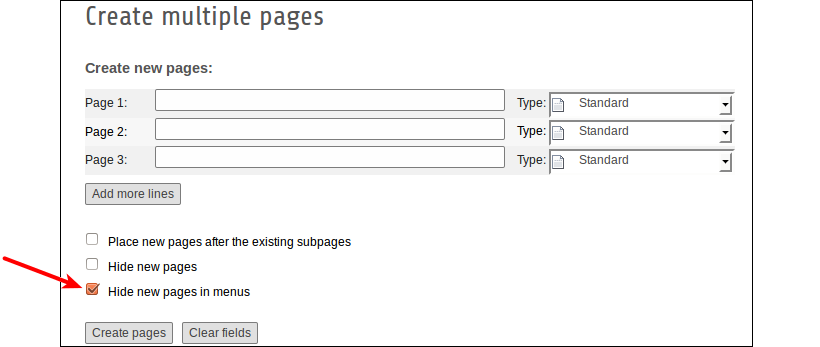
\includegraphics[width=0.85\linewidth]{Images/BackendChanges/CreateMultiplePagesHideInMenu.png}
	\end{figure}

\end{frame}

% ------------------------------------------------------------------------------
% Extension Manager: Upload Extensions
% ------------------------------------------------------------------------------
% http://forge.typo3.org/issues/51776
% http://forge.typo3.org/issues/51437

\begin{frame}[fragile]
	\frametitle{Backend Changes}
	\framesubtitle{Extension Manager}

 	\begin{itemize}
		\item Upload an extension via the "Get Extensions" function
	\end{itemize}

	\begin{figure}
		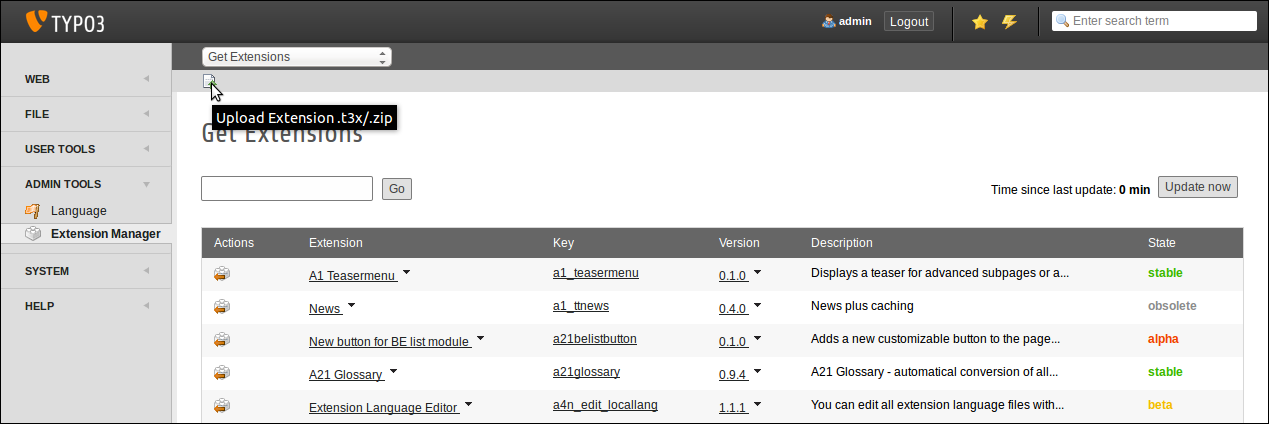
\includegraphics[width=0.95\linewidth]{Images/BackendChanges/UploadExtension.png}
	\end{figure}

\end{frame}

% ------------------------------------------------------------------------------
% Recycler
% ------------------------------------------------------------------------------
% http://forge.typo3.org/issues/52324

\begin{frame}[fragile]
	\frametitle{Backend Changes}
	\framesubtitle{Recycler}

 	\begin{itemize}
		\item Recycler records can be sorted by time stamp\newline
			\small(this helps users to decide whether to recover a specific record or not)\normalsize
	\end{itemize}

	\begin{figure}
		\includegraphics[width=0.95\linewidth]{Images/BackendChanges/RecyclerSortRecord.png}
	\end{figure}

\end{frame}

% ------------------------------------------------------------------------------
% File/Directory Permissions
% ------------------------------------------------------------------------------

\begin{frame}[fragile]
	\frametitle{Backend Changes}
	\framesubtitle{File/Directory Permissions}

 	\begin{itemize}
		\item Much more granular file/directory permissions for BE users/groups
			\begingroup\color{typo3red}\textbf{(1)}\endgroup
		\item This is possible since TYPO3 6.0, but only via UserTSconfig
			\begingroup\color{typo3red}\textbf{(2)}\endgroup
	\end{itemize}

	\begin{figure}
		\includegraphics[width=0.75\linewidth]{Images/BackendChanges/FileAndDirectoryPermissions.png}
	\end{figure}

\end{frame}

% ------------------------------------------------------------------------------
% OpenID
% ------------------------------------------------------------------------------

\begin{frame}[fragile]
	\frametitle{Backend Changes}
	\framesubtitle{OpenID (1)}

 	\begin{itemize}
		\item OpenID for BE user authentication can be configured by using a wizard
		\item EXT:openid (system extension) is required for this feature
	\end{itemize}

	\begin{figure}
		\includegraphics[width=0.95\linewidth]{Images/BackendChanges/OpenIdWizard.png}
	\end{figure}

\end{frame}

% ------------------------------------------------------------------------------
% OpenID
% ------------------------------------------------------------------------------

\begin{frame}[fragile]
	\frametitle{Backend Changes}
	\framesubtitle{OpenID (2)}

 	\begin{itemize}
		\item OpenID for BE user authentication can be configured by using a wizard
		\item EXT:openid (system extension) is required for this feature
	\end{itemize}

	\begin{figure}
		\includegraphics[width=0.8\linewidth]{Images/BackendChanges/OpenIdLogin.png}
	\end{figure}

 	\begin{itemize}
		\item Further details about OpenID:\newline
			\small\url{http://openid.net}\normalsize
	\end{itemize}

\end{frame}

% ------------------------------------------------------------------------------
% Workspaces
% ------------------------------------------------------------------------------
% http://forge.typo3.org/issues/50223
% http://forge.typo3.org/issues/50224

\begin{frame}[fragile]
	\frametitle{Backend Changes}
	\framesubtitle{Workspaces}

 	\begin{itemize}
		\item Editors/users can define who to notify, without limiting this on the system level
		\item Tab "All" is now visible to \underline{all} users
	\end{itemize}

	\begin{figure}
		\includegraphics[width=0.95\linewidth]{Images/BackendChanges/WorkspacesTabAll.png}
	\end{figure}

\end{frame}

% ------------------------------------------------------------------------------



% ------------------------------------------------------------------------------
% Chapter 4: TypoScript
% ------------------------------------------------------------------------------

% ------------------------------------------------------------------------------
% TYPO3 CMS 7.2 - What's New - Chapter "TypoScript" (English Version)
%
% @author	Michael Schams <schams.net>
% @license	Creative Commons BY-NC-SA 3.0
% @link		http://typo3.org/download/release-notes/whats-new/
% @language	English
% ------------------------------------------------------------------------------
% LTXE-CHAPTER-UID:		12518a77-2b90a173-4e3f8420-485e0497
% LTXE-CHAPTER-NAME:	TypoScript
% ------------------------------------------------------------------------------
% LTXE-SLIDE-START
% LTXE-SLIDE-UID:		56b025e6-cf380b11-c9d1c009-0b548d6a
% LTXE-SLIDE-TITLE:		Add flexible preview URL configuration (1)
% LTXE-SLIDE-REFERENCE:	Feature-66370-AddFlexiblePreviewUrlConfiguration.rst
% ------------------------------------------------------------------------------
\begin{frame}[fragile]
	\frametitle{TSconfig \& TypoScript}
	\framesubtitle{Flexible Preview URL Configuration (1)}

	% decrease font size for code listing
	\lstset{basicstyle=\tiny\ttfamily}

	\begin{itemize}

		\item It is now possible to configure the preview link generated for the\newline
			"save \& view" button in the backend.

		\item A common use case is to have previews for blog or news records, but you
			can also define different preview pages for normal content elements.

			\begin{lstlisting}
				TCEMAIN.preview {
				  <table name> {
				    previewPageId = 123
				    useDefaultLanguageRecord = 0
				    fieldToParameterMap {
				      uid = tx_myext_pi1[showUid]
				    }
				    additionalGetParameters {
				      tx_myext_pi1[special] = HELLO
				    }
				  }
				}
			\end{lstlisting}

	\end{itemize}

\end{frame}

% ------------------------------------------------------------------------------
% LTXE-SLIDE-START
% LTXE-SLIDE-UID:		6822c376-37649cd8-0acc836a-b856fc61
% LTXE-SLIDE-TITLE:		Add flexible preview URL configuration (2)
% LTXE-SLIDE-REFERENCE:	Feature-66370-AddFlexiblePreviewUrlConfiguration.rst
% ------------------------------------------------------------------------------
\begin{frame}[fragile]
	\frametitle{TSconfig \& TypoScript}
	\framesubtitle{Flexible Preview URL Configuration (2)}

	\begin{itemize}
		\item \texttt{previewPageId}:\newline
			\smaller
				UID of the page to use for preview\newline
				(if this setting is omitted the current page will be used)
			\normalsize
		\item \texttt{useDefaultLanguageRecord}:\newline
			\smaller
				defines if translated records will use the UID of the default record\newline
				(this is activated by default, value: 1)
			\normalsize
		\item \texttt{fieldToParameterMap}:\newline
			\smaller
				a mapping which allows to select fields of the record to be included as GET-parameters
			\normalsize
		\item \texttt{additionalGetParameters}:\newline
			\smaller
				allows to add arbitrary GET-parameters and even to override others
			\normalsize
	\end{itemize}

\end{frame}

% ------------------------------------------------------------------------------
% LTXE-SLIDE-START
% LTXE-SLIDE-UID:		c5dbf3c7-655fc6e4-227a3bf6-f5d89fb1
% LTXE-SLIDE-TITLE:
% LTXE-SLIDE-REFERENCE:	Feature-59646-AddRteConfigurationPropertyButtonsLinkTypePropertiesTargetDefault.rst
% ------------------------------------------------------------------------------
\begin{frame}[fragile]
	\frametitle{TSconfig \& TypoScript}
	\framesubtitle{RTE Configuration: Default Target}

	\begin{itemize}

		\item RTE configuration property can be used in PageTSconfig to configure a default
			target for links of a given type\newline

			\small
				\texttt{buttons.link.[}
				\textit{type}
				\texttt{].properties.target.default = ...}
			\normalsize\newline

		\item Possible link types are:\newline
			\small
				(further types may be provided by extensions)
			\normalsize

			\begin{itemize}
				\item \texttt{page}
				\item \texttt{file}
				\item \texttt{url}
				\item \texttt{mail}
				\item \texttt{spec}
			\end{itemize}
	\end{itemize}

\end{frame}

% ------------------------------------------------------------------------------
% LTXE-SLIDE-START
% LTXE-SLIDE-UID:		fd957580-301e4a0a-ad5325f5-ffa024c3
% LTXE-SLIDE-TITLE:		Strip empty HTML tags in HtmlParser
% LTXE-SLIDE-REFERENCE:	Feature-20555-StripEmptyHtmlTags.rst
% ------------------------------------------------------------------------------
\begin{frame}[fragile]
	\frametitle{TSconfig \& TypoScript}
	\framesubtitle{Strip Empty HTML Tags in HTMLparser}

	% decrease font size for code listing
	\lstset{basicstyle=\tiny\ttfamily}

	\begin{itemize}
		\item A new functionality has been implemented in the HTMLparser that allows the
			stripping of empty HTML tags

			\begin{lstlisting}
				stdWrap {
				   // this removes all empty HTML tags
				   HTMLparser.stripEmptyTags = 1
				   // this removes empty h2 and h3 tags only
				   HTMLparser.stripEmptyTags.tags = h2, h3
				}

				RTE.default.proc.entryHTMLparser_db {
				   stripEmptyTags = 1
				   stripEmptyTags.tags = p
				   stripEmptyTags.treatNonBreakingSpaceAsEmpty = 1
				}
			\end{lstlisting}

			\underline{\textbf{Note:}}
				HTMLparser strips all unknown tags by default.\newline
				Therefore it might be useful to retain these:\newline
				\texttt{HTMLparser.keepNonMatchedTags = 1}

	\end{itemize}

\end{frame}

% ------------------------------------------------------------------------------
% LTXE-SLIDE-START
% LTXE-SLIDE-UID:		62960e76-c3dca953-fe5a1070-831633fc
% LTXE-SLIDE-TITLE:		Miscellaneous
% LTXE-SLIDE-REFERENCE:	Feature-63040-AddRteConfigurationPropertyButtonsAbbreviationRemoveFieldsets.rst
% LTXE-SLIDE-REFERENCE:	commit 31c62f9311ee3d33bf792d548cc4a5fac83aa3d0
% ------------------------------------------------------------------------------
\begin{frame}[fragile]
	\frametitle{TSconfig \& TypoScript}
	\framesubtitle{Miscellaneous}

	\begin{itemize}
		\item New property \texttt{buttons.abbreviation.removeFieldsets} may be used in
			PageTSconfig to configure the abbreviation dialog

			\begin{lstlisting}
				# Possible values are:
				# acronym, definedAcronym, abbreviation, definedAbbreviation
				buttons.abbreviation.removeFieldsets = acronym,definedAcronym
			\end{lstlisting}

		\item Property \texttt{inlineLanguageLabel} of object \texttt{PAGE} can handle\newline
			\texttt{LLL:} references now

	\end{itemize}

\end{frame}

% ------------------------------------------------------------------------------


% ------------------------------------------------------------------------------
% Chapter 5: Package Management
% ------------------------------------------------------------------------------

% ------------------------------------------------------------------------------
% TYPO3 CMS 6.2 LTS - What's New - Chapter "Package Management" (Serbian Version)
%
% @author	Sinisa Mitrovic <mitrovic.sinisaa@gmail.com>
% @license	Creative Commons BY-NC-SA 3.0
% @link		http://typo3.org/download/release-notes/whats-new/
% @language	Serbian
% ------------------------------------------------------------------------------
% Chapter: Package Management
% ------------------------------------------------------------------------------

\section{Package Management}
\begin{frame}[fragile]
	\frametitle{Package Management}

	\begin{center}\huge{Poglavlje 5:}\end{center}
	\begin{center}\huge{\color{typo3darkgrey}\textbf{Package Management}}\end{center}

\end{frame}

% ------------------------------------------------------------------------------
% Package Manager
% ------------------------------------------------------------------------------
% http://wiki.typo3.org/Blueprints/Packagemanager
% http://forge.typo3.org/issues/47018
% http://forge.typo3.org/issues/52737

	\begin{frame}[fragile]
	\frametitle{Package Management}
	\framesubtitle{Package Manager}

	\begin{itemize}
		\item \textbf{Package Manager} iz Typo3 Flow je uveden u Typo3 CMS
		\item Razvoj/istrazivanje zapoceto je za vreme razvijanja TYPO3 CMS 6.1 verzije
		\item Ovaj projekat ima za cilj da uskladi formate razlicitih paketa
		\item Prosirenja u TYPO3 CMS su samo specificni tipovi paketa ("Packages")
		\item Glavni ciljevi projekta:

			\begin{itemize}
				\item Odgovarajuci API za Package Management
				\item Vendor Namespace podrska
				\item Composer Package podrska
				\item Flow Package podrska
				\item Autoloader Re-factoring
			\end{itemize}

	\end{itemize}

\end{frame}

% ------------------------------------------------------------------------------
% Package Manager Integration
% ------------------------------------------------------------------------------

\begin{frame}[fragile]
	\frametitle{Package Management}
	\framesubtitle{Implementacija Package Manager-a}

	\begin{itemize}
		\item Uklonjen je \texttt{\$TYPO3\_CONF['EXT']['extListArray']} iz fajla: \newline
			\smaller\texttt{typo3conf/LocalConfiguration.php}\normalsize

		\item Stari sadrzaj fajla \small\texttt{typo3conf/LocalConfiguration.php} prekopiran je u \normalsize\newline
			\smaller\texttt{typo3conf/LocalConfiguration.beforePackageStatesMigration.php}\normalsize

		\item Fajl \texttt{typo3conf/PackageStates.php} sadrzi:

			\begin{itemize}
				\item stanje paketa (aktivno/neaktivno)
				\item lokacija prosirenja u fajl sistemu
			\end{itemize}

		\item Prosirenja iz sledecih direktorijuma se prepoznaju automatski:

			\begin{itemize}
				\item \texttt{typo3/sysext/}
				\item \texttt{typo3/ext/}
				\item \texttt{typo3/contrib/}
				\item \texttt{typo3conf/ext/}
				\item \texttt{Packages/} \emph{(rekurzivno)}
			\end{itemize}

	\end{itemize}

\end{frame}

% ------------------------------------------------------------------------------
% Package Manager Integration
% ------------------------------------------------------------------------------

\begin{frame}[fragile]
	\frametitle{Package Management}
	\framesubtitle{Implementacija Package Manager-a}

	\begin{itemize}

		\item Dva nova (dodatna) fajla u direktorijumu prosirenja:

			\begin{itemize}
				\item \texttt{composer.json}
				\item \texttt{Classes/Package.php}
			\end{itemize}

		\item Ukoliko je prosirenje neophodno, oznaka \texttt{protected}\newline
			se postavlja u fajlu \texttt{composer.json}

		\item Ukoliko fajl \texttt{PackageStates.php} on ce biti (ponovno) kreiran\newline
			i sadrzace sva prosirenja kojima je gore navedena osobina podesena na \texttt{TRUE}

		\item Autoloader dobija sopstveni administrativni panel koji se kesira

		\item Dodatne informacije:\newline
			\url{http://wiki.typo3.org/Blueprints/Packagemanager}

	\end{itemize}

\end{frame}

% ------------------------------------------------------------------------------
% Examples
% ------------------------------------------------------------------------------

\begin{frame}[fragile]
	\frametitle{Package Management}
	\framesubtitle{Implementacija Package Manager-a}

	Primer: \texttt{typo3conf/PackageManager.php}

	\lstset{
		basicstyle=\tiny\ttfamily
		% basicstyle=\fontsize{5}{7}\selectfont\ttfamily
	}

	\begin{lstlisting}
		return array ('packages' =>
		    array (
		      'core' =>
		        array (
		          'manifestPath' => '',
		          'composerName' => 'typo3/cms/core',
		          'state' => 'active',
		          'packagePath' => 'typo3/sysext/core/',
		          'classesPath' => 'Classes/',
		        ),
		      'workspaces' =>
		        array (
		          'manifestPath' => '',
		          'composerName' => 'typo3/cms/workspaces',
		          'state' => 'inactive',
		          'packagePath' => 'typo3/sysext/workspaces/',
		          'classesPath' => 'Classes/',
		        ),
		      ...
		    ),
		    'version' => 4,
		);
	\end{lstlisting}

\end{frame}

% ------------------------------------------------------------------------------
% Examples
% ------------------------------------------------------------------------------

\begin{frame}[fragile]
	\frametitle{Package Management}
	\framesubtitle{Implementacija Package Manager-a}

	Primer: \texttt{composer.json}

	\lstset{
		basicstyle=\tiny\ttfamily
	}

	\begin{lstlisting}
		{
		  "name": "typo3/cms-indexed-search",
		  "type": "typo3-cms-framework",
		  "description": "TYPO3 Core",
		  "homepage": "http://typo3.org",
		  "license": ["GPL-2.0+"],
		  "version": "6.2.0",
		  "require": {
		    "typo3/cms-core": "*"
		  },
		  "replace": {
		    "indexed_search": "*"
		  }
		}
	\end{lstlisting}

\end{frame}

% ------------------------------------------------------------------------------
% Miscellaneous
% (slide added in March 2014)
% ------------------------------------------------------------------------------

\begin{frame}[fragile]
	\frametitle{Package Management}
	\framesubtitle{Implementacija Package Manager-a}

	\lstset{
		basicstyle=\smaller\ttfamily
	}

	\begin{itemize}
		\item Paketi se takodje mogu aktivirati za vreme rada uz pomoc kljuca:
			\smaller\texttt{\$GLOBALS['TYPO3\_CONF\_VARS']['EXT']['runtimeActivatedPackages'] = array(}\space\textit{packageKey}\space\texttt{);}\normalsize

		\item Ovaj kljuc se aktivira odmah nakon inicijalizacije Package Management-a

	\end{itemize}

\end{frame}

% ------------------------------------------------------------------------------



% ------------------------------------------------------------------------------
% Chapter 6: In-Depth Changes
% ------------------------------------------------------------------------------

% ------------------------------------------------------------------------------
% TYPO3 CMS 7.6 - What's New - Chapter "In-Depth Changes" (Greek Version)
%
% @author	Angeliki Plati <ag.plati@gmail.com>
% @license	Creative Commons BY-NC-SA 3.0
% @link		http://typo3.org/download/release-notes/whats-new/
% @language	Greek
% ------------------------------------------------------------------------------
% LTXE-CHAPTER-UID:		7229f1b9-b481e9bc-09c46183-a86b6a7e
% LTXE-CHAPTER-NAME:	In-Depth Changes
% ------------------------------------------------------------------------------

\section{\greektext ������� �������}
\begin{frame}[fragile]
	\frametitle{\greektext ������� �������}

	\begin{center}\huge{\greektext �������� 3:}\end{center}
	\begin{center}\huge{\color{typo3darkgrey}\textbf{\greektext ������� �������}}\end{center}

\end{frame}

% ------------------------------------------------------------------------------
% LTXE-SLIDE-START
% LTXE-SLIDE-UID:		fb7f39e9-a9c3b856-0f20d933-42501d14
% LTXE-SLIDE-ORIGIN:	159a2d7f-b679989c-30cf1736-6693f827 English
% LTXE-SLIDE-TITLE:		Bootstrap for Install Tool (1)
% ------------------------------------------------------------------------------

\begin{frame}[fragile]
	\frametitle{\greektext ������� �������}
	\framesubtitle{\latintext Bootstrap \greektext ��� �� \latintext Install Tool (1)}

	\begin{itemize}

		\item \greektext �� \latintext Install Tool \greektext ��������� ���� ��� \latintext Bootstrap - \greektext
		��� �� ������� ��� ������������:

			\latintext\begin{figure}
				\includegraphics[width=0.7\linewidth]{InDepthChanges/InstallToolBootstrap01.jpg}
			\end{figure}

	\end{itemize}

\end{frame}

% ------------------------------------------------------------------------------
% LTXE-SLIDE-START
% LTXE-SLIDE-UID:		57b94677-df4363dd-e5477dbf-04d344c7
% LTXE-SLIDE-ORIGIN:	66a71f73-91b6c90e-e548a037-e2d47f94 English
% LTXE-SLIDE-TITLE:		Bootstrap for Install Tool (2)
% ------------------------------------------------------------------------------

\begin{frame}[fragile]
	\frametitle{\greektext ������� �������}
	\framesubtitle{\latintext Bootstrap \greektext ��� �� \latintext Install Tool (2)}

	\begin{itemize}

		\item \greektext �� \latintext Install Tool \greektext ��������� ���� ��� \latintext Bootstrap - \greektext ��� ���
		 ���������� \latintext(configuration):

			\latintext\latintext\begin{figure}
				\includegraphics[width=0.7\linewidth]{InDepthChanges/InstallToolBootstrap02.png}
			\end{figure}

	\end{itemize}

\end{frame}

% ------------------------------------------------------------------------------
% LTXE-SLIDE-START
% LTXE-SLIDE-UID:		5c40f730-3d75f880-2c050954-902634a3
% LTXE-SLIDE-ORIGIN:	f901074a-4080140f-dd93e505-1e8c2178 English
% LTXE-SLIDE-ORIGIN:	d5acb2d2-159a2d7f-6693f827-30cf1736 German
% LTXE-SLIDE-TITLE:		Form protection API for frontend usage
% LTXE-SLIDE-REFERENCE:	Feature-56633-FormProtectionAPIForFrontEndUsage.rst
% ------------------------------------------------------------------------------

\begin{frame}[fragile]
	\frametitle{\greektext ������� �������}
	\framesubtitle{\greektext ��������� \latintext CSRF \greektext ��� �� \latintext Frontend Plugins}

	% decrease font size for code listing
	\lstset{basicstyle=\tiny\ttfamily}

	\begin{itemize}

		\item \greektext ��� ����� ��������� �� ����� ��� \latintext FormProtection API \greektext ��� \latintext frontend

		\item \greektext ���� �������� ��� ��������� \latintext CSRF (Cross-Site Request Forgery)

			\latintext\begin{lstlisting}
				$formToken = \TYPO3\CMS\Core\FormProtection\FormProtectionFactory::get()->getFormProtection()->generateToken('news', 'edit', $uid);
				if (
				  $dataHasBeenSubmitted
				  && \TYPO3\CMS\Core\FormProtection\FormProtectionFactory::get()->validateToken(
				    \TYPO3\CMS\Core\Utility\GeneralUtility::_POST('formToken'), 'User setup', 'edit')) {
				  // processes the data
				}
				else {
				  // invalid token!
				}
			\end{lstlisting}

	\end{itemize}

\end{frame}

% ------------------------------------------------------------------------------
% LTXE-SLIDE-START
% LTXE-SLIDE-UID:		a5c1d7d5-a793018d-2463f644-1502b46d
% LTXE-SLIDE-ORIGIN:	0198b067-68da7843-6a6d3f6d-94cee9b7 English
% LTXE-SLIDE-ORIGIN:	388c7243-b679989c-e2b30dbb-78f1aea4 German
% LTXE-SLIDE-TITLE:		Added LinkBrowser APIs (1)
% LTXE-SLIDE-REFERENCE:	Feature-66369-AddedLinkBrowserAPIs.rst
% ------------------------------------------------------------------------------

\begin{frame}[fragile]
	\frametitle{\greektext ������� �������}
	\framesubtitle{\latintext Tabs \greektext ��� ��� \latintext LinkBrowser (1)}

	% decrease font size for code listing
	\lstset{basicstyle=\tiny\ttfamily}

	\begin{itemize}

		\item \greektext ���� �� ��� ������������� ��������� ��� �������� ���
		\latintext LinkBrowser \greektext �� ��� \latintext tabs

		\item \greektext K��� \latintext tab \greektext ����� ��� �� ���������� ���� \latintext "LinkHandler", \greektext
		� ������ ������ �� �������� ��� �������� ������� \latintext (Interface):\newline
			\latintext\small
				\texttt{\textbackslash TYPO3\textbackslash CMS\textbackslash Recordlist\textbackslash LinkHandler\textbackslash LinkHandlerInterface}
			\normalsize

		\item \greektext �� \latintext LinkHandlers \greektext ����� ������������� ��� \latintext PageTSconfig \greektext �� ����:

			\latintext\begin{lstlisting}
				file {
				  handler = TYPO3\\CMS\\Recordlist\\LinkHandler\\FileLinkHandler
				  label = LLL:EXT:lang/locallang_browse_links.xlf:file
				  displayAfter = page
				  scanAfter = page
				  configuration {
				    customConfig = passed to the handler
				  }
				}
			\end{lstlisting}

	\end{itemize}

\end{frame}

% ------------------------------------------------------------------------------
% LTXE-SLIDE-START
% LTXE-SLIDE-UID:		e30adb51-b7f5a42f-e8d02ad3-b31f0cce
% LTXE-SLIDE-ORIGIN:	7ff322bc-2ace574c-34ddebb5-559fd90c English
% LTXE-SLIDE-ORIGIN:	dfd89b4b-7b4b816c-e5904ba8-2527339b German
% LTXE-SLIDE-TITLE:		Added LinkBrowser APIs (2)
% LTXE-SLIDE-REFERENCE:	Feature-66369-AddedLinkBrowserAPIs.rst
% ------------------------------------------------------------------------------

\begin{frame}[fragile]
	\frametitle{\greektext ������� �������}
	\framesubtitle{\latintext Tabs \greektext ��� ��� \latintext (2)}

	% decrease font size for code listing
	\lstset{basicstyle=\tiny\ttfamily}

	\begin{itemize}

		\item \greektext �� �������� \latintext \texttt{displayBefore} \greektext ��� \latintext \texttt{displayAfter}
		\greektext ���������� ��� ������ ��� \latintext tabs

		\item \greektext �� �������� \latintext \texttt{scanBefore} \greektext ��� \latintext \texttt{scanAfter} \greektext
		���������� �� ����� �� ��� ����� �� \latintext handlers \greektext ����������� ���� ���������� ���������� ���������

			\latintext\begin{lstlisting}
				$GLOBALS['TYPO3_CONF_VARS']['SC_OPTIONS']['LinkBrowser']['hooks'][1444048118] = [
				  'handler' => \Vendor\Ext\MyClass::class,
				  'before' => [], // optional
				  'after' => [] // optional
				];
			\end{lstlisting}

	\end{itemize}

\end{frame}

% ------------------------------------------------------------------------------
% LTXE-SLIDE-START
% LTXE-SLIDE-UID:		146ef043-c98a5f26-dcc6c06d-42bf0733
% LTXE-SLIDE-ORIGIN:	1ef90646-4f4342dd-3bf0112b-95acba1b English
% LTXE-SLIDE-ORIGIN:	687f24a3-032124a3-7ac41f15-26329962 German
% LTXE-SLIDE-TITLE:		Module Template API (1)
% LTXE-SLIDE-REFERENCE:	Feature-69814-ModuleTemplateAPI.rst
% ------------------------------------------------------------------------------

\begin{frame}[fragile]
	\frametitle{\greektext ������� �������}
	\framesubtitle{Module Template API (1)}

	% decrease font size for code listing
	\lstset{basicstyle=\tiny\ttfamily}

	\begin{itemize}

		\item \greektext ��� ��� \latintext Module Template API \greektext ���� �� ����� ��� �������������� ��� ����������
		��� \latintext DocHeaders

		\item \greektext ���������� 1: �������� ���� ��������

			\latintext\begin{lstlisting}
				$openInNewWindowButton = $this->moduleTemplate->getDocHeaderComponent()->getButtonBar()
				  ->makeLinkButton()
				  ->setHref('#')
				  ->setTitle($this->getLanguageService()->sL(
				    'LLL:EXT:lang/locallang_core.xlf:labels.openInNewWindow', TRUE
				    ))
				  ->setIcon($this->iconFactory->getIcon('actions-window-open', Icon::SIZE_SMALL))
				  ->setOnClick($aOnClick);

				$this->moduleTemplate->getDocHeaderComponent()->getButtonBar()
				  ->addButton($openInNewWindowButton, ButtonBar::BUTTON_POSITION_RIGHT);
			\end{lstlisting}
	\end{itemize}

\end{frame}

% ------------------------------------------------------------------------------
% LTXE-SLIDE-START
% LTXE-SLIDE-UID:		61fbcc28-5b90c26b-1613c13c-60a90ea0
% LTXE-SLIDE-ORIGIN:	44c8e88e-5668ccb6-3cf424ea-c6a40ecf English
% LTXE-SLIDE-ORIGIN:	1570c8c9-2dfa48e9-058d2d04-bff5465d German
% LTXE-SLIDE-TITLE:		Module Template API (2)
% LTXE-SLIDE-REFERENCE:	Feature-69814-ModuleTemplateAPI.rst
% ------------------------------------------------------------------------------

\begin{frame}[fragile]
	\frametitle{\greektext ������� �������}
	\framesubtitle{Module Template API (2)}

	% decrease font size for code listing
	\lstset{basicstyle=\tiny\ttfamily}

	\begin{itemize}
		\item \greektext ���������� 2: �������� ���� ����� �� �������� �����

			\latintext\begin{lstlisting}
				$languageMenu = $this->moduleTemplate->getDocHeaderComponent()
				  ->getModuleMenuRegistry()->makeMenu()
				  ->setIdentifier('_langSelector')
				  ->setLabel($this->getLanguageService()->sL(
				    'LLL:EXT:lang/locallang_general.xlf:LGL.language', TRUE
				  ));

				$menuItem = $languageMenu->makeMenuItem()
				  ->setTitle($lang['title'] . $newTranslation)
				  ->setHref($href);

				if((int)$lang['uid'] === $currentLanguage) {
				  $menuItem->setActive(TRUE);
				}

				$languageMenu->addMenuItem($menuItem);
				$this->moduleTemplate->getDocHeaderComponent()->getModuleMenuRegistry()->addMenu($languageMenu);
			\end{lstlisting}
	\end{itemize}

\end{frame}


% ------------------------------------------------------------------------------
% LTXE-SLIDE-START
% LTXE-SLIDE-UID:		168df078-18d15bd7-9a74f411-a271e50a
% LTXE-SLIDE-ORIGIN:	2ffbc623-117a44dc-923610ec-78a3afc2 English
% LTXE-SLIDE-ORIGIN:	df3ea848-d5406e98-edbd6684-485ff477 German
% LTXE-SLIDE-TITLE:		PSR-7-based Routing for Backend AJAX Requests
% LTXE-SLIDE-REFERENCE:	Feature-69916-PSR-7-basedRoutingForBackendAJAXRequests.rst
% ------------------------------------------------------------------------------

\begin{frame}[fragile]
	\frametitle{\greektext ������� �������}
	\framesubtitle{\greektext ����������� \latintext PSR-7 \greektext ��� \latintext Backend AJAX Requests}

	% decrease font size for code listing
	\lstset{basicstyle=\tiny\ttfamily}

	\begin{itemize}

		\item \greektext ��� ��� �������� ���� ��������� ��� ��� \latintext AJAX request, \greektext �� ������
			\latintext\texttt{Configuration/Backend/AjaxRoutes.php}\newline
			\greektext ������ �� ������������ �� �� �������� �����������:

			\latintext\begin{lstlisting}
				return [
				  // do something
				  'unique_route_name' => [
				    'path' => '/toolcollection/some-action',
				    'target' => \Vendor\Controller\SomeController::class . '::myAction',
				  ]
				];
			\end{lstlisting}

	\end{itemize}

\end{frame}

% ------------------------------------------------------------------------------
% LTXE-SLIDE-START
% LTXE-SLIDE-UID:		67138f5a-0623c3ab-1acbe95a-f121e37c
% LTXE-SLIDE-ORIGIN:	b68a9d26-30e6d4a0-7bccecf2-ad1f93c6 English
% LTXE-SLIDE-ORIGIN:	cb01cca6-58e91977-d18fa0b3-cba021ab German
% LTXE-SLIDE-TITLE:		Introduced two new Hooks for OpenID (getUserRecord)
% LTXE-SLIDE-REFERENCE:	Feature-44127-HooksForOpenIdToAutomaticallyCreateUserAccounts.rst
% ------------------------------------------------------------------------------
\begin{frame}[fragile]
	\frametitle{\greektext ������� �������}
	\framesubtitle{\latintext OpenID \greektext �������� \latintext (Hook) \texttt{getUserRecord}}

	% decrease font size for code listing
	\lstset{basicstyle=\tiny\ttfamily}

	\greektext ��� �������� ����� ��������� ��� \latintext OpenID service (1/2)

		\begin{itemize}

			\item \greektext �������� 1:\newline
				\smaller\smaller
					\latintext\texttt{\$GLOBALS['TYPO3\_CONF\_VARS']['SC\_OPTIONS']['openid']['getUserRecord']}
				\normalsize

				\begin{itemize}
					\item \greektext ���������� ��� ������� ������ ���� ���� ������������, �:
					\item \greektext ���������� ��� ��� ������� �� �� ������� �����
					\item \greektext �� ���������� \latintext\texttt{record}, \texttt{response} \greektext ��� \latintext \texttt{authInfo} \greektext
					������������ ��� ��������
				\end{itemize}

		\end{itemize}

\end{frame}

% ------------------------------------------------------------------------------
% LTXE-SLIDE-START
% LTXE-SLIDE-UID:		7854fdf6-584fdd28-988ab41d-9283e206
% LTXE-SLIDE-ORIGIN:	b9b259e4-9d35ace7-edff1014-7390d1d1 English
% LTXE-SLIDE-ORIGIN:	ea0bfed8-831666d7-1ba40bb9-7a95723a German
% LTXE-SLIDE-TITLE:		Introduced two new Hooks for OpenID (authRequest)
% LTXE-SLIDE-REFERENCE:	Feature-44127-HooksForOpenIdToAutomaticallyCreateUserAccounts.rst
% ------------------------------------------------------------------------------
\begin{frame}[fragile]
	\frametitle{\greektext ������� �������}
	\framesubtitle{\greektext �������� \latintext (Hook) \texttt{authRequest}}

	% decrease font size for code listing
	\lstset{basicstyle=\tiny\ttfamily}

	\greektext ��� �������� ����� ��������� ��� \latintext OpenID service (2/2)

		\begin{itemize}

			\item \greektext �������� 2:\newline
				\latintext\smaller\smaller
					\texttt{\$GLOBALS['TYPO3\_CONF\_VARS']['SC\_OPTIONS']['openid']['authRequest']}
				\normalsize

				\begin{itemize}
					\item \greektext ���������� �� \latintext Authentication Request, \greektext ���� ���� ������
					\item \greektext ������ �� �������������� ��� �� \latintext request \greektext ������������ ���������
					���� ��� \latintext nickname \greektext ��� ��� \latintext OpenID Server \greektext ��� ����������
					\item \greektext �� ���������� \latintext \texttt{authRequest} \greektext ��� \latintext \texttt{authInfo}
					\greektext ������������ ��� ��������
				\end{itemize}

		\end{itemize}

\end{frame}

% ------------------------------------------------------------------------------
% LTXE-SLIDE-START
% LTXE-SLIDE-UID:		d6cd9df0-bd81dbae-51c9a744-7f157bb5
% LTXE-SLIDE-ORIGIN:	1626edc6-8d93ff84-f64178bf-8e7650df English
% LTXE-SLIDE-ORIGIN:	115a4459-3653bb99-1680d6ab-d8c3c69b German
% LTXE-SLIDE-TITLE:		Hook in BackendUserAuthentication::getDefaultUploadFolder (1)
% LTXE-SLIDE-REFERENCE:	Feature-68895-IntroducedHookInBackendUserAuthenticationgetDefaultUploadFolder.rst
% ------------------------------------------------------------------------------
\begin{frame}[fragile]
	\frametitle{\greektext ������� �������}
	\framesubtitle{\greektext �������� ��� ������ (1)}

	% decrease font size for code listing
	\lstset{basicstyle=\tiny\ttfamily}

	\begin{itemize}

		\item \greektext ����� ���� ������ �� ������� ������ ��� ������ \latintext upload \greektext
		 ��� ������������ ��� ��� \latintext
			\texttt{BackendUserAuthentication::getDefaultUploadFolder()}

		\item \greektext � ������� ��� ��������� ��� ������ \latintext \texttt{ext\_localconf.php} \greektext ������� �� ����:

			\latintext\begin{lstlisting}
				$GLOBALS['TYPO3_CONF_VARS']['SC_OPTIONS']['t3lib/class.t3lib_userauthgroup.php']
				  ['getDefaultUploadFolder'][] =
				  \Vendor\MyExtension\Hooks\DefaultUploadFolder::class . '->getDefaultUploadFolder';
			\end{lstlisting}

	\end{itemize}

\end{frame}

% ------------------------------------------------------------------------------
% LTXE-SLIDE-START
% LTXE-SLIDE-UID:		e3b6ef85-9b24f220-ee6cb871-28d33337
% LTXE-SLIDE-ORIGIN:	9c150d50-ee3ba19b-120ef653-e714135c English
% LTXE-SLIDE-ORIGIN:	d1041967-32814ee3-2172e570-4a6d21bd German
% LTXE-SLIDE-TITLE:		Hook in BackendUserAuthentication::getDefaultUploadFolder (2)
% LTXE-SLIDE-REFERENCE:	Feature-68895-IntroducedHookInBackendUserAuthenticationgetDefaultUploadFolder.rst
% ------------------------------------------------------------------------------
\begin{frame}[fragile]
	\frametitle{\greektext ������� �������}
	\framesubtitle{\greektext �������� ��� ������ (2)}

	% decrease font size for code listing
	\lstset{basicstyle=\tiny\ttfamily}

	\small \greektext ����������:\normalsize

		\latintext\begin{lstlisting}
			<?php
			namespace Vendor\MyExtension\Hooks;
			use TYPO3\CMS\Core\Authentication\BackendUserAuthentication;
			use TYPO3\CMS\Core\Resource\Folder;

			/**
			 * Class DefaultUploadFolder
			 */
			class DefaultUploadFolder {

			  /**
			   * Get default upload folder
			   * If there is a folder present with the same name as the last part of the table name use that folder.
			   * @param array $params
			   * @param BackendUserAuthentication $backendUserAuthentication
			   * @return Folder
			   */
			   public function getDefaultUploadFolder($params, BackendUserAuthentication $backendUserAuthentication) {
			    [...]
		\end{lstlisting}

\end{frame}

% ------------------------------------------------------------------------------
% LTXE-SLIDE-START
% LTXE-SLIDE-UID:		3403e92e-1bb3a37a-b53a812c-c1b7bbdb
% LTXE-SLIDE-ORIGIN:	a4d7bec0-6c19d8b2-6a6be951-5d5aa0c0 English
% LTXE-SLIDE-ORIGIN:	2f855107-2262065c-c865f953-91b4f0ea German
% LTXE-SLIDE-TITLE:		Hook in BackendUserAuthentication::getDefaultUploadFolder (3)
% LTXE-SLIDE-REFERENCE:	Feature-68895-IntroducedHookInBackendUserAuthenticationgetDefaultUploadFolder.rst
% ------------------------------------------------------------------------------
\begin{frame}[fragile]
	\frametitle{\greektext ������� �������}
	\framesubtitle{\greektext �������� ��� ������ (3)}

	% decrease font size for code listing
	\lstset{basicstyle=\tiny\ttfamily}

	\small \greektext ���������� (��������):\normalsize

		\latintext\begin{lstlisting}
			    [...]

			    /** @var Folder $uploadFolder */
			    $uploadFolder = $params['uploadFolder'];
			    $pid = $params['pid'];
			    $table = $params['table'];
			    $field = $params['field'];

			    $matches = [];
			    if (!empty($uploadFolder) && preg_match('/_([a-z]+)$/', $table, $matches)) {
			      $folderName = $matches[1];
			      if ($uploadFolder->hasFolder($folderName)) {
			        $uploadFolder = $uploadFolder->getSubfolder($folderName);
			      }
			    }
			    return $uploadFolder;
			  }
			}
		\end{lstlisting}

\end{frame}

% ------------------------------------------------------------------------------
% LTXE-SLIDE-START
% LTXE-SLIDE-UID:		498d8f09-18df23db-2a659e1c-cf467bca
% LTXE-SLIDE-ORIGIN:	2c656d9e-38b9be7a-d590cb6e-21eccd4d English
% LTXE-SLIDE-ORIGIN:	cd6ba83d-9f068dee-b8887ffa-4a2eff29 German
% LTXE-SLIDE-TITLE:		Diverse ?nderungen
% LTXE-SLIDE-REFERENCE:	Deprecation-69822-DeprecateSelectFieldTca.rst
% ------------------------------------------------------------------------------
\begin{frame}[fragile]
	\frametitle{\greektext ������� �������}
	\framesubtitle{\greektext �������}

	\begin{itemize}

		\item \greektext � ����� ��� ����� ������ \latintext TCA \texttt{select} \greektext ������� ��� ������������ ���� ��������
		 \latintext\texttt{renderType}

		\item \greektext ������� ����� �����:

			\latintext\begin{lstlisting}
				'renderType' => 'selectMultipleSideBySide',
				'renderType' => 'selectCheckBox',
				'renderType' => 'selectSingle',
				'renderType' => 'selectSingleBox',
				'renderType' => 'selectTree',
			\end{lstlisting}

	\end{itemize}

\end{frame}

% ------------------------------------------------------------------------------


% ------------------------------------------------------------------------------
% Chapter 7: Application Programming Interface
% ------------------------------------------------------------------------------

% ------------------------------------------------------------------------------
% TYPO3 CMS 6.2 LTS - What's New - Chapter "Application Programming Interface" (Dutch version)
%
% @author	Christiaan Wiesenekker <cwiesenekker@gmail.com>
% @author	Ric van Westhreenen <ric.vanwesthreenen@typo3.org>
% @license	Creative Commons BY-NC-SA 3.0
% @link		http://typo3.org/download/release-notes/whats-new/
% @language	Dutch
% ------------------------------------------------------------------------------
% Chapter: Application Programming Interface
% ------------------------------------------------------------------------------

\section{Application Programming Interface}
\begin{frame}[fragile]
	\frametitle{Application Programming Interface}

	\begin{center}\huge{Hoofdstuk 6:}\end{center}
	\begin{center}\huge{\color{typo3darkgrey}\textbf{Application Programming Interface (API)}}\end{center}

\end{frame}

% ------------------------------------------------------------------------------
% Hook: tsfe::checkEnableFields
% ------------------------------------------------------------------------------
% http://forge.typo3.org/issues/48981

\begin{frame}[fragile]
	\frametitle{Application Programming Interface}
	\framesubtitle{Hook: \texttt{tsfe::checkEnableFields}}

	\begin{itemize}
		\item In TYPO3 < 6.2, "\emph{breid uit naar subpagina's}" kan niet worden gebruikt in eigen extensies die extra regels hebben voor pagina zichtbaarheid\newline
			\small(lijst van velden om te controleren is hard-coded in \texttt{tsfe::checkEnableFields()})\normalsize

		\item In TYPO3 >= 6.2, een nieuwe hook staat het extensies toe om nieuwe regels toe te maken voor pagina zichtbaarheid wanneer 'parent pages' when parent pages "extend to subpages" hebben geactiveerd.
		\item Class:\newline
			\smaller
				\texttt{\textbackslash
					TYPO3\textbackslash
					CMS\textbackslash
					Frontend\textbackslash
					Controller\textbackslash
					TypoScriptFrontendController}\normalsize

			\lstset{
				basicstyle=\smaller\ttfamily
			}

			\begin{lstlisting}
				$GLOBALS['TYPO3_CONF_VARS']['SC_OPTIONS']
				  ['tslib/class.tslib_fe.php']['hook_checkEnableFields']
			\end{lstlisting}

	\end{itemize}

\end{frame}

% ------------------------------------------------------------------------------
% Hook: checkFlexFormValue in DataHandler
% ------------------------------------------------------------------------------
% http://forge.typo3.org/issues/49699

\begin{frame}[fragile]
	\frametitle{Application Programming Interface}
	\framesubtitle{Hook: \texttt{checkFlexFormValue} in DataHandler}

	\begin{itemize}
		\item In TYPO3 < 6.2, wanneer je de Flexform waardes update, is er geen controle of er een bestaande waarde in de database ook echt is verwijderd. 
		\item Dit wordt een probleem, e.g. wanneer je switchable controller actions opslaat (Extbase) in de Flexform: oude acties die niet meer aanwezig mogen zijn moeten handmatig worden verwijderd

		\item In TYPO3 >= 6.2, een nieuwe hook staat het to om de oude Flexform data aan te passen voor het wordt gemerged met de nieuwe
		\item Class:\newline
			\smaller
				\texttt{\textbackslash
					TYPO3\textbackslash
					CMS\textbackslash
					Core\textbackslash
					DataHandling\textbackslash
					DataHandler}\normalsize

			\lstset{
				basicstyle=\smaller\ttfamily
			}

			\begin{lstlisting}
				$GLOBALS['TYPO3_CONF_VARS']['SC_OPTIONS']
				  ['t3lib/class.t3lib_tcemain.php']['checkFlexFormValue']
			\end{lstlisting}

		\item Method:\newline
			\smaller
				\texttt{checkFlexFormValue\_beforeMerge()}

	\end{itemize}

\end{frame}

% ------------------------------------------------------------------------------
% Hook to customize header in module "Web > Page"
% ------------------------------------------------------------------------------
% http://forge.typo3.org/issues/52579

\begin{frame}[fragile]
	\frametitle{Application Programming Interface}
	\framesubtitle{Hook om de header aan te passen}

	\begin{itemize}
		\item In TYPO3 >= 6.2, een nieuwe hook maakt het mogelijk om de header van een pagina aan te passen in de page module (Module: "Web > Page")
		\item De hook wordt aangeroepen voor de content van de pagina wordt gerendered.
		\item Class:\newline
			\smaller
				\texttt{\textbackslash
					TYPO3\textbackslash
					CMS\textbackslash
					Backend\textbackslash
					Controller\textbackslash
					PageLayoutController}\normalsize

			\lstset{
				basicstyle=\smaller\ttfamily
			}

			\begin{lstlisting}
				$GLOBALS['TYPO3_CONF_VARS']['SC_OPTIONS']
				  ['cms/layout/db_layout.php']['drawHeaderHook']
			\end{lstlisting}

		\item Method:\newline
			\smaller
				\texttt{callUserFunction()}

	\end{itemize}

\end{frame}

% ------------------------------------------------------------------------------
% IRRE: Provide default values for created records
% ------------------------------------------------------------------------------
% http://forge.typo3.org/issues/46124

\begin{frame}[fragile]
	\frametitle{Application Programming Interface}
	\framesubtitle{IRRE: standaard waardes voor gecreeerde records}

	\begin{itemize}
		\item De nieuwe TCA optie staat het to om "inline" fields in te stellen
		\item Key \texttt{foreign\_record\_defaults} staat het toe om (default) waardes in nieuwe gecreeerde records in te stellen

			\begin{lstlisting}
				config => array(
				  'type' => 'inline',
				  'foreign_table' => 'tt_content',
				  'foreign_record_defaults' => array(
				    'CType' => 'image'
				  ),
				)
			\end{lstlisting}

			\small
				Voorbeeld hierboven: \texttt{tt\_content} elementen die zijn gecreeerd voor dit IRRE veld worden standaard \textbf{image content elements}. De editor kan dit andere type instellen voor het opslaan.
			\normalsize

	\end{itemize}

\end{frame}

% ------------------------------------------------------------------------------
% Workspaces
% ------------------------------------------------------------------------------
% http://forge.typo3.org/issues/46124

\begin{frame}[fragile]
	\frametitle{Application Programming Interface}
	\framesubtitle{Workspaces (1)}

	\begin{itemize}
		\item In TYPO3 < 6.2, de module "Workspaces" kan alleen worden uitgebreid door het overschrijven van de PHP en JavaScript componenten
		\item In TYPO3 >= 6.2, is het nu mogelijk om de definitie en het gedrag van de getoonde kolommen uit te breiden in de module
		\item Een paar voorbeelden op de volgende slides...
	\end{itemize}

\end{frame}

% ------------------------------------------------------------------------------
% Workspaces
% ------------------------------------------------------------------------------
% http://forge.typo3.org/issues/46124

\begin{frame}[fragile]
	\frametitle{Application Programming Interface}
	\framesubtitle{Workspaces (2)}

	\lstset{
		basicstyle=\tiny\ttfamily
	}

	Voorbeeld 1 (file \texttt{ext\_localconf.php}):

	\begin{lstlisting}
		$GLOBALS['TYPO3_CONF_VARS']['SC_OPTIONS']
		  ['t3lib/class.t3lib_tcemain.php']['processCmdmapClass']['workspaces_logger'] =
		  'Vendor\\WorkspacesLogger\\Hook\\DataHandlerHook';
	\end{lstlisting}

	Voorbeeld 2 (file \texttt{ext\_tables.php}):

	\begin{lstlisting}
		\TYPO3\CMS\Workspaces\Service\AdditionalColumnService::getInstance()->register(
		  'WorkspacesLogger_StageChange',
		  'Vendor\\WorkspacesLogger\\DataProvider'
		);

		\TYPO3\CMS\Workspaces\Service\AdditionalResourceService::getInstance()->addJavaScriptResource(
		  'WorkspacesLogger',
		  'EXT:myextension/Resources/Public/JavaScript/StageChange.js'
		);
	\end{lstlisting}

\end{frame}

% ------------------------------------------------------------------------------
% Workspaces
% ------------------------------------------------------------------------------
% http://forge.typo3.org/issues/46124

\begin{frame}[fragile]
	\frametitle{Application Programming Interface}
	\framesubtitle{Workspaces (3)}

	Voorbeeld (file \texttt{Vendor\textbackslash
		WorkspacesLogger\textbackslash
		Hook\textbackslash
		DataHandlerHook}):

	\lstset{
		basicstyle=\tiny\ttfamily
	}

	\begin{lstlisting}
		<?php
		namespace Vendor\WorkspacesLogger\Hook;
		use TYPO3\CMS\Core\SingletonInterface;

		class DataHandlerHook implements SingletonInterface {

		  const TABLE_Name = 'tx_workspaceslogger_event';
		  const EVENT_SetStage = 91;

		  /**
		   * hook that is called when no prepared command was found
		   */
		  public function processCmdmap($command, $table, $id, $value, &$commandIsProcessed,
		    \TYPO3\CMS\Core\DataHandling\DataHandler $tcemainObj) {
		    ...
		    $action = (string) $value['action'];
		    if ($command === 'version' && $action === 'setStage' && $commandIsProcessed) {
		      ...
		    }
		  }
		}
	\end{lstlisting}

\end{frame}

% ------------------------------------------------------------------------------
% PSR-3 compatible Logger
% ------------------------------------------------------------------------------
% http://forge.typo3.org/issues/48880

\begin{frame}[fragile]
	\frametitle{Application Programming Interface}
	\framesubtitle{PSR-3 compatible Logger}

	\begin{itemize}
		\item De TYPO3 CMS 6.2 logging API is nu PSR-3 compatible
		\item PSR-3 richt zich op het maken van een standaard voor logging in PHP (standard of the PHP Framework Interop Group)

		\item Het hoofddoel van PSR-3 is
			"\emph{libraries toestaan tot het ontvangen van een LoggerInterface object en de logs er naar toe te schrijven in een eenvoudige en op een universele manier.}"

		\item Logger interface bevat snelle log methoden zoals\newline
			\texttt{debug()}, \texttt{warning()}, \texttt{notice()}, \texttt{alert()}, \texttt{error()}, etc.

		\item  Andere bronnen:
			\begin{itemize}
				\item \url{http://www.php-fig.org/psr/3/}
			\end{itemize}

	\end{itemize}

\end{frame}

% ------------------------------------------------------------------------------
% Miscellaneous
% ------------------------------------------------------------------------------
% http://forge.typo3.org/issues/49144 (MathUtility: Add canBeInterpretedAsFloat)
% http://forge.typo3.org/issues/52707 (Introduce a PHP Enumeration type)
% http://forge.typo3.org/issues/52762 (Add type converter for core types like Enumeration)

\begin{frame}[fragile]
	\frametitle{Application Programming Interface}
	\framesubtitle{Miscellaneous}

	\begin{itemize}
		\item Nieuwe methode \texttt{canBeInterpretedAsFloat()} in class: \texttt{MathUtility}\newline
			\small(Dit is een analogie van: \texttt{canBeInterpretedAsInteger()})\normalsize
		\item Nieuwe enumeration type (zonder relatie naar derde partij PHP modules):\newline
			\texttt{\textbackslash
				TYPO3\textbackslash
				CMS\textbackslash
				Core\textbackslash
				Type\textbackslash
				Enumeration}\newline

			Als voorbeeld gebruikt in in:\newline
			\texttt{\textbackslash
				TYPO3\textbackslash
				CMS\textbackslash
				Core\textbackslash
				Versioning\textbackslash
				VersionState}\newline

			...en dan als:\newline
			\texttt{new VersionState(VersionState::DEFAULT\_STATE);}

	\end{itemize}

\end{frame}

% ------------------------------------------------------------------------------



% ------------------------------------------------------------------------------
% Chapter 8: Extbase & Fluid
% ------------------------------------------------------------------------------

% ------------------------------------------------------------------------------
% TYPO3 CMS 8.5 - What's New - Chapter "Extbase & Fluid" (German Version)
%
% @author	Michael Schams <schams.net>
% @license	Creative Commons BY-NC-SA 3.0
% @link		http://typo3.org/download/release-notes/whats-new/
% @language	English
% ------------------------------------------------------------------------------
% LTXE-CHAPTER-UID:		846d40ce-66fdc2ec-750dcf95-33ce93e0
% LTXE-CHAPTER-NAME:	Extbase & Fluid
% ------------------------------------------------------------------------------

\section{Extbase \& Fluid}
\begin{frame}[fragile]
	\frametitle{Extbase \& Fluid}

	\begin{center}\huge{Kapitel 4:}\end{center}
	\begin{center}\huge{\color{typo3darkgrey}\textbf{Extbase \& Fluid}}\end{center}

\end{frame}

% ------------------------------------------------------------------------------
% LTXE-SLIDE-START
% LTXE-SLIDE-UID:		506eeccc-87f8f148-a064b4e2-121d876f
% LTXE-SLIDE-ORIGIN:	c5986329-fb36f473-a5430d2e-6ba49fb1 English
% LTXE-SLIDE-TITLE:		#78116: Extbase support for Doctrine's native DBAL Statement and QueryBuilder
% ------------------------------------------------------------------------------
\begin{frame}[fragile]
	\frametitle{Extbase \& Fluid}
	\framesubtitle{Doctrine DBAL}

	% decrease font size for code listing
	\lstset{basicstyle=\tiny\ttfamily}

	\begin{itemize}
		\item Die Möglichkeit direkt SQL-Queries abzusetzen, unterstützt nun auch QueryBuilder-Objekte und Instanzen von 
			\texttt{\textbackslash
			Doctrine\textbackslash
			DBAL\textbackslash
			Statement} als "Prepared Statements"
		\item Das folgende Beispiel zeigt die Anwendung über eine Repository und mittels einem nativem Doctrine DBAL Statement:

			\begin{lstlisting}
				$connection = $this->objectManager->get(ConnectionPool::class)->getConnectionForTable('mytable');
				$statement = $this->objectManager->get(
				  \Doctrine\DBAL\Statement::class,
				  'SELECT * FROM mytable WHERE uid=? OR title=?',
				  $connection
				);

				$query = $this->createQuery();
				$query->statement($statement, [$uid, $title]);
			\end{lstlisting}
	\end{itemize}

\end{frame}
% ------------------------------------------------------------------------------
% LTXE-SLIDE-START
% LTXE-SLIDE-UID:		76b41536-ec795de9-6197748f-5d429230
% LTXE-SLIDE-ORIGIN:	8d31d436-4397d4fd-aa0eed2e-df798aa3 English
% LTXE-SLIDE-TITLE:		#78002: Enforce cHash argument for Extbase actions
% ------------------------------------------------------------------------------

\begin{frame}[fragile]
	\frametitle{Extbase \& Fluid}
	\framesubtitle{\texttt{cHash} Argument}

	\begin{itemize}
		\item URLS zu Extbase-Actions benötigen nun per default einen gültigen\texttt{cHash}\newline
			(für gechachte und ungecachte Actions)
		\item Dieses Verhalten kann über den Typoscript \texttt{feature} Switch abgeschaltet werden:
			\texttt{requireCHashArgumentForActionArguments}
	\end{itemize}

\end{frame}
% ------------------------------------------------------------------------------
% LTXE-SLIDE-START
% LTXE-SLIDE-UID:		80792903-9dd8a7ed-355eca78-479cea5e
% LTXE-SLIDE-ORIGIN:	50143a1e-53a17c8c-83ffe7ea-5e88cba0 English
% LTXE-SLIDE-TITLE:		#29399: OptionViewHelper and OptgroupViewHelper
% ------------------------------------------------------------------------------

\begin{frame}[fragile]
	\frametitle{Extbase \& Fluid}
	\framesubtitle{Inhalt für ViewHelper \texttt{f:form.select}}

	% decrease font size for code listing
	\lstset{basicstyle=\tiny\ttfamily}

	\begin{itemize}
		\item Es wurden zwei neue ViewHelper eingeführt, welche die manuelle Definition aller Optionen und Optionen-Gruppen für den \texttt{f:form.select} ViewHelper als Tag-Inhalt zulässt

			\begin{itemize}
				\item \texttt{OptionViewHelper}
				\item \texttt{OptgroupViewHelper}
			\end{itemize}

		\item Beispiel:

			\begin{lstlisting}
				<f:form.select name="myproperty">
				  <f:form.select.option value="1">Option one</f:form.select.option>
				  <f:form.select.option value="2">Option two</f:form.select.option>
				  <f:form.select.optgroup>
				    <f:form.select.option value="3">Grouped option one</f:form.select.option>
				    <f:form.select.option value="4">Grouped option twi</f:form.select.option>
				  </f:form.select.optgroup>
				</f:form.select>
			\end{lstlisting}

		\end{itemize}

\end{frame}


% ------------------------------------------------------------------------------
% LTXE-SLIDE-START
% LTXE-SLIDE-UID:		45ba8a94-0ddf9140-b871dc35-f0040ec2
% LTXE-SLIDE-ORIGIN:	d36b9935-fc7d9e60-742a3f42-ef15e856 English
% LTXE-SLIDE-TITLE:		#78415: Global Fluid ViewHelper Namespace
% ------------------------------------------------------------------------------
\begin{frame}[fragile]
	\frametitle{Extbase \& Fluid}
	\framesubtitle{Globaler Fluid ViewHelper Namespace}

	\begin{itemize}
		\item Der globale Fluid ViewHelper Namespace sind nun konfigurierbar:\newline
			\smaller
				\texttt{\$GLOBALS['TYPO3\_CONF\_VARS']['SYS']['fluid']['namespaces']}
			\normalsize
		\item Dies erlaubt die Manipulation der Namespaces auf der Ebene der Seitenkonfiguration
		\item Vorteile:

			\begin{itemize}
				\item Third-Party ViewHelper Pakete können nun den globalen Fluid Namespace \texttt{f:} manipulieren
				\item Third-Party ViewHelper Pakete können nun neue globale Namespaces registrieren
				\item Template-Entwickler können solche globale Namespace in allen Fluid Template (kontextunabhängig) verwenden, ohne diese vorher zu importieren.
			\end{itemize}

	\end{itemize}

\end{frame}


% ------------------------------------------------------------------------------
% LTXE-SLIDE-START
% LTXE-SLIDE-UID:		f3f97fb5-c9c96120-9b45756f-74d08679
% LTXE-SLIDE-ORIGIN:	e16e8cfd-26f35f09-23b473a2-442ff1e2 English
% LTXE-SLIDE-TITLE:		#78842: FLUIDTEMPLATE can mimic an actual Extbase web request
% ------------------------------------------------------------------------------
\begin{frame}[fragile]
	\frametitle{Extbase \& Fluid}
	\framesubtitle{\texttt{FLUIDTEMPLATE} kann Extbase Web Requests nachahmen}

	% decrease font size for code listing
	\lstset{basicstyle=\small\ttfamily}

	\begin{itemize}
		\item Das \texttt{FLUIDTEMPLATE} Content-Element kann nun einen Extbase Web Request nachahmen.
		\item Damit kann man z.B. auf übermittelte Daten zugreifen:

			\begin{lstlisting}
				$view->getRenderingContext()
				  ->getControllerContext()
				  ->getRequest()
				  ->getArguments();
			\end{lstlisting}

	\end{itemize}

\end{frame}




% ------------------------------------------------------------------------------


% ------------------------------------------------------------------------------
% Chapter 9: Upgrade TYPO3 CMS 4.5 to 6.2 LTS
% ------------------------------------------------------------------------------

% ------------------------------------------------------------------------------
% TYPO3 CMS 6.2 LTS - What's New - Chapter "Upgrade" (French Version)
%
% @author	Paul Blondiaux <pblondiaux@sodifrance.fr>
% @author	Philippe Herault <philippe.herault@plan-net.fr>
% @license	Creative Commons BY-NC-SA 3.0
% @link		http://typo3.org/download/release-notes/whats-new/
% @language	French
% ------------------------------------------------------------------------------
% Chapter: Upgrade to TYPO3 CMS 6.2 LTS
% ------------------------------------------------------------------------------

\section{Migration vers TYPO3 CMS 6.2 LTS}
\begin{frame}[fragile]
	\frametitle{Migration vers TYPO3 CMS 6.2 LTS}

	\begin{center}\huge{Chapitre 9 :}\end{center}
	\begin{center}\huge{\color{typo3darkgrey}\textbf{Migration vers TYPO3 CMS 6.2 LTS}}\end{center}

\end{frame}

% ------------------------------------------------------------------------------
% General Upgrade Instructions
% ------------------------------------------------------------------------------

\begin{frame}[fragile]
	\frametitle{Migration vers TYPO3 CMS 6.2 LTS}
	\framesubtitle{Instructions générales pour la migration}

	\begin{itemize}

		\item Instructions de migration :\newline
			\smaller\url{http://wiki.typo3.org/Upgrade#Upgrading_to_6.2}\normalsize
		\item Guide officiel TYPO3 « Installation et migration de TYPO3 » :
			\smaller\url{http://docs.typo3.org/typo3cms/InstallationGuide}\normalsize
				\item Approche générale :
			\begin{itemize}
				\item Vérifier si le système respecte la configuration requise \small(PHP, MySQL, etc.)\normalsize
				\item Reconsidérer le \textbf{deprecation\_*.log} dans l'ancienne instance TYPO3
				\item Mettre à jour toutes les extensions\newline
					\small(vérifier la compatibilité avec TYPO3 6.2)\normalsize
				\item Voir le chapitre « Install Tool » dans cette présentation
			\end{itemize}
	\end{itemize}

\end{frame}

% ------------------------------------------------------------------------------
% Upgrade from TYPO3 CMS 4.5 LTS
% ------------------------------------------------------------------------------

\begin{frame}[fragile]
	\frametitle{Migration vers TYPO3 CMS 6.2 LTS}	
	\framesubtitle{Migration à partir d'un TYPO3 CMS 4.5 LTS}

	\begin{itemize}
		\item De nombreux sites TYPO3 passeront d'une LTS à la LTS suivante
		\item Le projet « Smooth Migration » :

			\begin{itemize}
				\item Pour qu'une migration d'une 4.5 à une 6.2 soit aussi douce que possible
				\item Documentation, identification des anomalies sur les extensions, etc.
				\item \smaller\url{http://forge.typo3.org/projects/typo3cms-smoothmigration}\normalsize
			\end{itemize}

		\item EXT:typo3-upgradereport :

			\begin{itemize}
				\item Principalement développée par Steffen Ritter
				\item Installer dans une instance de TYPO3 CMS 4.5 LTS et lancer les tests
				\item Participer au développement
				\item \smaller\url{https://github.com/nxpthx/typo3-upgradereport}\normalsize
			\end{itemize}
	\end{itemize}

\end{frame}

% ------------------------------------------------------------------------------
% What's New for Editors
% ------------------------------------------------------------------------------

\begin{frame}[fragile]
	\frametitle{Migration vers TYPO3 CMS 6.2 LTS}
	\framesubtitle{What's New for Editors}

	\begin{itemize}
		\item Résume les principaux changements entre TYPO3 CMS 4.5 et 6.2
		\item Public cible : principalement des éditeurs (utilisateurs peu ou pas techniques)
		\item Vise aussi à aider les agences :

			\begin{itemize}
				\item dans la préparation des réponses aux demandes de support
				\item dans l'animation d'ateliers, séminaires, formations, etc.
			\end{itemize}

		\item Télécharger le document « \textbf{What's New for Editors} »:\newline
			\smaller\url{http://typo3.org/download/release-notes/whats-new}\normalsize

	\end{itemize}

\end{frame}

% ------------------------------------------------------------------------------



% ------------------------------------------------------------------------------
% Chapter 10: Myth Buster
% ------------------------------------------------------------------------------

% ------------------------------------------------------------------------------
% TYPO3 CMS 6.2 LTS - What's New - Chapter "MythBuster" (German Version)
%
% @author	Michael Schams <schams.net>
% @license	Creative Commons BY-NC-SA 3.0
% @link		http://typo3.org/download/release-notes/whats-new/
% @language	German
% ------------------------------------------------------------------------------
% Chapter: MythBuster
% ------------------------------------------------------------------------------

\section{MythBuster}
\begin{frame}[fragile]
	\frametitle{MythBuster}

	\begin{center}\huge{Kapitel 10:}\end{center}
	\begin{center}\huge{\color{typo3darkgrey}\textbf{TYPO3 CMS 6.2 LTS - MythBuster}}\end{center}

\end{frame}

% ------------------------------------------------------------------------------
% MythBuster
% ------------------------------------------------------------------------------

\begin{frame}[fragile]
	\frametitle{MythBuster}
	\framesubtitle{Mythen über TYPO3 CMS 6.2}

	\begin{itemize}
		\item TYPO3 CMS 6.2 LTS wird das letzte TYPO3 CMS Release sein
			\tabto{9cm}\color{red}\textbf{\textrightarrow falsch!}\color{black}

			\smaller
				Die Wahrheit ist, dass trotz der Veröffentlichung von \href{http://neos.typo3.org}{TYPO3 Neos} die Entwicklung von TYPO3 CMS fortgesetzt wird und dass es auch in Zukunft weitere Versionen geben wird.
			\normalsize
			\newline

		\item Der TYPO3 Core wurde in 6.x komplett überarbeitet
			\tabto{9cm}\color{red}\textbf{\textrightarrow falsch!}\color{black}

			\smaller
				Die Wahrheit ist, dass mit TYPO3 CMS 6.0 das PHP Konzept von "\href{http://php.net/namespaces}{Namespaces}" eingeführt wurde, was neue Klassennamen zur Folge hat. Allerdings stellt eine Kompatibilitäts- schicht in TYPO3 sicher, dass Entwickler noch weiterhin die bisherigen, veralteten Klassennamen ohne Probleme in ihren Extensions verwenden können.
			\normalsize

	\end{itemize}

\end{frame}

% ------------------------------------------------------------------------------
% MythBuster
% ------------------------------------------------------------------------------

\begin{frame}[fragile]
	\frametitle{MythBuster}
	\framesubtitle{Mythen über TYPO3 CMS 6.2}

	\begin{itemize}

		\item Extensions, die für TYPO3 CMS 4.5 entwickelt wurden,\newline
			funktionieren in 6.2 nicht mehr\tabto{9cm}\color{red}\textbf{\textrightarrow falsch!}\color{black}

			\smaller
				Die Wahrheit ist, dass die Core API nicht vollständig geändert wurde und eine Abwärtskompatibilität aufweist, die der \href{http://forge.typo3.org/projects/typo3v4-core/wiki/CoreDevPolicy}{Deprecation Policy} entspricht. Die meisten Extensions, die für TYPO3 CMS 4.5 entwickelt wurden, sind auch in TYPO3 CMS 6.2 lauffähig, ohne dass Modifikationen notwendig sind (oder nur geringe Anpassungen).
			\normalsize
			\newline

		\item TemplaVoilà ist in TYPO3 6.2 nicht mehr lauffähig
			\tabto{9cm}\color{red}\textbf{\textrightarrow falsch!}\color{black}

			\smaller
				Die Wahrheit ist, dass die Entwicklergemeinschaft an einer Version von TemplaVoilà arbeitet, die auch mit TYPO3 CMS 6.2 kompatibel ist. Allerdings wird TemplaVoilà nicht weiterentwickelt und TYPO3 Integratoren sollten für zukünftige Projekte Alternativen in Erwägung ziehen.
			\normalsize

	\end{itemize}

\end{frame}

% ------------------------------------------------------------------------------
% MythBuster
% ------------------------------------------------------------------------------

\begin{frame}[fragile]
	\frametitle{MythBuster}
	\framesubtitle{Mythen über TYPO3 CMS 6.2}

	\begin{itemize}

		\item \texttt{tslib\_pibase}-Extensions funktionieren nicht mehr
			\tabto{9cm}\color{red}\textbf{\textrightarrow falsch!}\color{black}

			\smaller
				Die Wahrheit ist, dass die Klasse \texttt{tslib\_pibase} auch in TYPO3 6.2 existiert, aber aufgrund der zuvor erwähnten Namespace-Konvention einen neuen Namen trägt: \texttt{\textbackslash TYPO3\textbackslash CMS\textbackslash Frontend\textbackslash Plugin\textbackslash AbstractPlugin}.\newline
				Ein Klassenalias stellt sicher, dass auch der bisherige Name verwendet werden kann (Abwärtkompatibilität).
			\normalsize
			\newline

		\item DAM Records können nicht nach FAL migriert werden
			\tabto{9cm}\color{red}\textbf{\textrightarrow falsch!}\color{black}

			\smaller
				Fakt ist, dass DAM nicht von TYPO3 6.x unterstützt wird. Allerdings bietet FAL eine API, die dazu bestimmt ist, sämtliche DAM-Funktionalität abzubilden. Es gibt außerdem eine \href{https://github.com/fnagel/t3ext-dam_falmigration}{DAM-to-FAL Migration Extension}.
			\normalsize

	\end{itemize}

\end{frame}

% ------------------------------------------------------------------------------
% MythBuster
% ------------------------------------------------------------------------------

\begin{frame}[fragile]
	\frametitle{MythBuster}
	\framesubtitle{Mythen über TYPO3 CMS 6.2}

	\begin{itemize}
		\item Upgrade von 4.5 zu 6.2 mit einem Upgrade-Wizard
			\tabto{9cm}\color{red}\textbf{\textrightarrow falsch!}\color{black}

			\smaller
				Gerüchten zufolge soll das "Smooth Migration" Projekt einen Upgrade-Wizard bereit stellen, der eine TYPO3 Version 4.5 automatisch zu 6.2 aktualisiert. Die Wahrheit ist, dass das Projekt das Ziel verfolgt, Information und Dokumentationen zu liefern, um TYPO3 Integratoren bei dem Migrationsprozess zu unterstützen.
			\normalsize
			\newline

		\item TYPO3 6.2 benötigt wesentlich bessere Hardware
			\tabto{9cm}\color{red}\textbf{\textrightarrow falsch!}\color{black}

			\smaller
				Gerüchten zufolge soll TYPO3 6.2 zehn Mal langsamer als 4.5 sein. Die Wahrheit ist, dass die Performance in den meisten Fällen identisch ist und sich die \href{http://typo3.org/about/typo3-the-cms/system-requirements/}{Mindestanforderungen} von TYPO3 CMS kaum geändert haben. Allerdings sollten Systemadministratoren einen Hardware-Upgrade generell in Erwägung ziehen, da TYPO3 4.5 bereits im Januar 2011 veröffentlicht wurde - also vor über 3 Jahren!
			\normalsize

	\end{itemize}

\end{frame}

% ------------------------------------------------------------------------------



% ------------------------------------------------------------------------------
% Chapter 11: Sources and Authors
% ------------------------------------------------------------------------------

% ------------------------------------------------------------------------------
% TYPO3 CMS 7.4 - What's New - Chapter "Sources" (English Version)
%
% @author	Michael Schams <schams.net>
% @license	Creative Commons BY-NC-SA 3.0
% @link		http://typo3.org/download/release-notes/whats-new/
% @language	English
% ------------------------------------------------------------------------------
% LTXE-CHAPTER-UID:		28e9cd26-94a5e6d3-1e306e2c-966ab751
% LTXE-CHAPTER-NAME:	Sources and Authors
% ------------------------------------------------------------------------------

\section{Sources and Authors}
\begin{frame}[fragile]
	\frametitle{Sources and Authors}

	\begin{center}\huge{Chapter 7:}\end{center}
	\begin{center}\huge{\color{typo3darkgrey}\textbf{Sources and Authors}}\end{center}

\end{frame}

% ------------------------------------------------------------------------------
% LTXE-SLIDE-START
% LTXE-SLIDE-UID:		fadfa59c-938d8b9b-bb000b6a-2c3e2337
% LTXE-SLIDE-ORIGIN:	8a9c5c3a-5742833d-83727e6e-c29f6991 German
% LTXE-SLIDE-TITLE:		Sources
% ------------------------------------------------------------------------------

\begin{frame}[fragile]
	\frametitle{Sources and Authors}
	\framesubtitle{Sources}

	\textbf{TYPO3 News:}
		\begin{itemize}\smaller
			\item \url{http://typo3.org/news}
		\end{itemize}

	\textbf{Release Infos:}
		\begin{itemize}\smaller
			\item \url{http://wiki.typo3.org/TYPO3_CMS_7.4.0}
			\item \href{https://github.com/TYPO3/TYPO3.CMS/blob/master/INSTALL.md}{INSTALL.md} and \href{https://github.com/TYPO3/TYPO3.CMS/blob/master/ChangeLog}{ChangeLog}
			\item \texttt{typo3/sysext/core/Documentation/Changelog/7.4/*}
		\end{itemize}

	\textbf{TYPO3 Bug-/Issuetracker:}
		\begin{itemize}\smaller
			\item \url{https://forge.typo3.org/projects/typo3cms-core}
		\end{itemize}

	\textbf{TYPO3 Git Repositories:}
		\begin{itemize}\smaller
			\item \url{https://git.typo3.org/Packages/TYPO3.CMS.git}
			\item \url{https://git.typo3.org/Packages/TYPO3.Fluid.git}
		\end{itemize}

\end{frame}

% ------------------------------------------------------------------------------
% LTXE-SLIDE-START
% LTXE-SLIDE-UID:		e18a2cb0-3c042a38-40f44a81-2dafa8cc
% LTXE-SLIDE-ORIGIN:	ba8cba39-772a4102-adeca680-5d9345a2 German
% LTXE-SLIDE-TITLE:		Authors
% ------------------------------------------------------------------------------

\begin{frame}[fragile]
	\frametitle{Sources and Authors}

	\vspace{-0.6cm}

	\centerline{\textbf{TYPO3 CMS What's New Slides:}}

	\begin{center}
		\smaller
			\centerline{Patrick Lobacher}
			\centerline{(Research, Information Gathering and German Version)}
			\vspace{0.1cm}
			\centerline{Michael Schams}
			\centerline{(Project Leader and English Version)}
		\normalsize
	\end{center}
	\vspace{-0.6cm}
	\begin{center}
		\smaller
			\centerline{\textbf{Translations by:}}
			\centerline{Andrey Aksenov, Paul Blondiaux, Pierrick Caillon, Sergio Catala, Jigal van Hemert, Michel Mix,}
			\centerline{Sinisa Mitrovic, Angeliki Plati, Nena Jelena Radovic, Roberto Torresani}
		\normalsize
	\end{center}
	\vspace{-0.6cm}
	\smaller\begin{center}\url{http://typo3.org/download/release-notes/whats-new}\end{center}\normalsize

	\smaller\begin{center}Licensed under Creative Commons BY-NC-SA 3.0\end{center}\normalsize
	\begin{figure}\vspace*{-0.3cm}
		\includegraphics[width=1.4cm]{SourcesAndAuthors/CreativeCommons-BY-NC-SA.png}
	\end{figure}

\end{frame}

% ------------------------------------------------------------------------------


% ------------------------------------------------------------------------------
% an empty frame to enforce entries in the table of contents
%
% \section{Empty Frame}
% \begin{frame}
% \end{frame}
%
% ------------------------------------------------------------------------------
\end{document}

